\chapter{The genomics of the Slavic migration period, Early Middle Ages and their links to the present day}
\label{chapterlabel5}

\section{Introduction}

The Slavic peoples originated as a diverse network of tribal societies who lived in Central and Eastern Europe from the first Millennia AD \cite{barford2001early} and whose origin, although disputed, is thought to be Polesia (a marshy forested area straddling Poland, Belarus, Russiana and Ukraine) \cite{fouracre1995new}. Although various Roman and Greek sources refer to Slavs as \textit{Veneti} and \textit{Spori} as early as the 1st and 2nd centuries AD, the term `Slavs' was first used in writing by Roman bureaucrat Jordanes at the beginning of the 6th century after their attack on the Byzantine empire \cite{curta2006southeastern}. This era, known by historians as The Migration Period, was a period of European history, roughly between 375-568 AD after the fall of the Roman Empire \cite{halsall2007barbarian}, characterised by the large-scale movement of various peoples. The Migration Period began with the Huns moving into Eastern Europe at the end of the 4th Century, occupying an area including present-day Hungary and Romania. During the 5th century, various Germanic groups invaded and established a homeland across parts of the Western Roman Empire. This was followed by the expansion of Slavic populations into regions of low population density in the sixth century.

Across the next 2 centuries, these peoples had settled across large parts of Europe. In particular, the Early Slavs had expanded southwards into the Balkans and Alps \cite{barford2001early, brather2008archaologie, geary2003myth,gojda1991ancient}. It has been proposed that these migrations were key to forming the foundations of present-day Slavic (speaking) nations \cite{barford2001early}.  

By the beginning of the 12th century, Slavs constituted a large part of a number of many medieval Christian states across Europe. As from this time period, Slavs could be broadly split up in 3 groups: the Eastern Slavs as part of the Kievan Rus', Southern Slavs in the Bulgarian Empire, the Principality of Serbia, Kingdom of Croatia and the Banate of Bosnia, and Western Slavs in the Principality of Nitra, Great Moravia, the duchy of Bohemia and the Kingdom and Poland. In addition, Slavic settlement also occurred in the Eastern Alps; Slovenia, large parts of present-day Austria and Friul. 

The differentiation of Slavs into these 3 broad groups can still be seen today in the different language groups. Today 315 million people speak Slavic languages. Linguistic evidence suggests that they can be broadly split into 3 groups; Western Slavs (Poles, Czechs and Slovaks), Eastern Slavs (Ukrainians, Belarusians and Russians) and Southern Slavs (Croatians, Bulgarians, Slovenians, Bosnians, Macedonians, Montenegrins and Serbians) \cite{sussex2006slavic}. 

The history of the Slavic peoples can be artificially be split into 3 periods; Migration Period(~375AD - ~568AD), Early Middle Ages/High Middle Ages (~600AD - ~1250AD) and present-day. Although previous studies have investigated the genetics of the transitions between these periods, they have been relatively limited in their scope. Juras et al (2014) used uniparental mtDNA markers from ancient DNA samples from Poland to show continuity between both Roman Iron Age period (200 BC – 500 AD) and Medieval Age (1000–1400AD) with present-day Poles, Czechs and Slovaks \cite{Juras2014}. Whilst informative about sex-biased migrations, uniparental markers carry only a fraction of the information that autosomal markers do, and therefore may provide misleading or incomplete information about the relationship between present-day and ancient samples \cite{Shaw16122} (although see \cite{10.1080/10635150500234674}). For example, it is know that mtDNA and nuclear DNA may have different evolutionary histories and thus display discordant phylogenetic trees \cite{posth2017deeply}. 

Kushniarevich et al (2015) \cite{Kushniarevich23015} combined results from mtDNA, non-recombining Y and autosomal DNA to investigate the population structure of a wide range of present-day Balto-Slavic populations in order to understand the historical processes that have formed the present-day genetic structure. They proposed that admixture of incoming Slavic speakers during the Migration Period with the pre-existing substrate of regional genetic components, which differed between South, East and West Slavs. Using this evidence, they propose that the "cultural assimilation of indigenous populations by bearers of Slavic languages as a major mechanism of the spread of Slavic languages to the Balkan Peninsula".

More recently, Macháček et al (2021) \cite{MACHACEK2021105333} analysed ancient rune inscriptions on an animal bone from Lány, Czechia, dated to approximately 600AD. The bone is inscribed with Germanic runes. Finding Germanic runes in the context of Slavic peoples provides evidence of early interactions between Slavic and Germanic peoples. However, whether there was early genetic contact as well is yet to be determined. 

Several studies into present-day Slavic populations have detected signatures of admixture from East-Asia \cite{Hellenthal2014, pankratov2016east, MOSAIC_2019, maliarchuk2008origin, qin2015quantitating}. Whether or not these signals can be observed in ancient individuals is yet to be seen and could further refine the admixture date. For example, different admixture dates in different Slavic populations may reveal structure amongs present-day Slavs. 

Finally, several studies have used haplotype-based methods to explore the structure of present-day Slavic populations. Ralph and Coop \cite{RalphCoop2013} compared regions of IBD matching  across different European populations. They found a relatively high degree of IBD sharing among pairs of individuals from Eastern Europe, suggestive of expansion from a smaller, common source population. This expansion was tentatively estimated to between 0-1000AD. Consistent with estimates of a small population size, Hellenthal et al (2014) \cite{Hellenthal2014} inferred an excess of IBD-sharing among Eastern European individuals, albeit with a more constrained admixture data of 440 - 1080 CE. However, this could also be interpreted in terms of a small effective population size \cite{al2019estimating, ringbauer2017inferring}. 

Despite these efforts, no studies have integrated autosomal DNA from ancient and present-day samples whilst applying powerful haplotype-based methods to infer population structure, ancestry proportions and admixture events. Therefore in this chapter, I will analyse 17 new medium to high coverage whole ancient genomes from Czech Republic, spanning the Migration Period and Early Middle Ages. These are, to my knowledge, the first high-coverage whole ancient-genomes from Slavic I will merge the newly sequenced sampled alongside a detailed reference datatset of other ancient individuals and a large reference set of relevant present-day European individuals in order to understand their ancestry in the context of both present-day and ancient samples. In particular, I am interested in considering the following questions:

\begin{enumerate}
\item Can we gain an understanding of the geographical origins of the Slavic peoples from ancient DNA
\item Do the labels "Migration Period" and "Early Middle Ages" make sense from a genetic standpoint (i.e. do samples from either period cluster with another to the exclusion of the other)
\item Was there interactions between Germanic and Slavic peoples during the Early Migration Period. 
\item If so, what genetic differences can be observed between these periods? Are they characterised by admixture from outside sources? If so, what are these sources and can the admixture events be dated?
\item What is the relationship between the ancient samples and present-day day Slavic populations. Are they continuous?
\item Do the different ancient Slavic samples have different affinities to different present-day Slavic language groups?
\end{enumerate}


\section{Methods}

\subsection{Description of samples}

Whole-genome sequence data was generated from 17 ancient individuals. 

All newly sequenced samples are from Czechia, split across two different field sites. 

The newly sequenced samples are grouped into two temporal categories; 5 samples are from the Migration Period (348 AD - 504 AD) and 12 samples are from the later Early Middle Ages (724 AD - 995 AD). 

\begin{tabular}{l|l|r|l}
\hline
Code & Site & Date (AD) & Period\\
\hline
LIB5 & Břeclav – Líbivá & 348 & Migration period\\
\hline
LIB4 & Břeclav – Líbivá & 472 & Migration period\\
\hline
LIB12 & Břeclav – Líbivá & 475 & Migration period\\
\hline
LIB2 & Břeclav – Líbivá & 495 & Migration period\\
\hline
LIB3 & Břeclav – Líbivá & 509 & Migration period\\
\hline
LIB11 & Břeclav – Líbivá & 741 & Early Middle Ages\\
\hline
LIB7 & Břeclav – Líbivá & 830 & Early Middle Ages\\
\hline
POH11 & Pohansko – Lesní školka & 783 & Early Middle Ages\\
\hline
POH27 & Pohansko – Jizní Předhradí & 783 & Early Middle Ages\\
\hline
POH28 & Pohansko – Jizní Předhradí & 822 & Early Middle Ages\\
\hline
POH41 & Pohansko – Lesní školka & 875 & Early Middle Ages\\
\hline
POH13 & Pohansko – Lesní školka & 879 & Early Middle Ages\\
\hline
POH36 & Pohansko – Jizní Předhradí & 880 & Early Middle Ages\\
\hline
POH40 & Pohansko – Lesní školka & 950 & Early Middle Ages\\
\hline
POH3 & Pohansko – Lesní hrúd & 956 & Early Middle Ages\\
\hline
POH44 & Pohansko – Pohřebištĕ U Kostela & NA & Early Middle Ages\\
\hline
POH39 & Pohansko – Jizní Předhradí & 866 & Early Middle Ages\\
\hline
\end{tabular}

Apart from the age of the samples, the differentiation between the Migration Period and Early Middle Age samples can be determined via pottery (Z. Hofmanova, personal communication).  

Include details of processing. Read alignment, read filtering, ATLAS calling etc. 

\subsection{Ancient DNA processing}

I merged the 17 newly sequenced individuals with the reference data-sets A.1 to A.17 resulting in a total of 942 individuals in .bcf format with genotype likelihood data at 77,213,942 genome-wide SNPs. Data was then split into separate .bcf files for each chromosome and indexed using bcftools.

I followed the GLIMPSE \cite{rubinacci2021efficient} imputation and phasing pipeline (\url{https://odelaneau.github.io/GLIMPSE/tutorial_b38.html}) to generate genotype likelihoods and phased genotypes for each individual. For the reference panel, I used the 30x 1000 genomes dataset \cite{byrska2021high}, described in appendix A.5.  

GLIMPSE was chosen as it is the most efficient (in terms of time and memory) probabilistic phasing / imputation software available \cite{rubinacci2021efficient}. 

First, GLIMPSE chunk was used to split the present-day reference dataset into chunks. Default settings of --window-size 2000000 and --buffer-size 200000 were used, generating a total of 936 regions genome wide. Splitting the genome into regions for imputation jointly maximises computational efficiency and accuracy. For each region in turn, the target dataset consisting of phred-scaled genotype likelihoods (PL) was imputed using GLIMPSE phase under default settings and the same reference panel. GLIMPSE ligate was then used to concatenate the 936 imputed regions into 22 distinct chromosomes. Finally, GLIMPSE sample was used to created phased haplotypes from the output of GLIMPSE ligate using default settings.

Previous sections (cite section) have shown that using a set of SNPs which are common yields results which are least affected by coverage related bias, likely in part because common variants are easier to impute. Therefore, I chose to filter the SNPs to those 477,416 those present in the HellBus dataset (A.20). Thus these SNPs were used for all subsequent analyses. 

\subsection{present-day DNA processing}

I chose the MS-POBI-HellBus dataset, described in detail in appendix A.20, because it contains a high number of relevant samples from central and Eastern Europe. I removed samples from Australia, New Zealand and USA, as these samples were not from native individuals from that country.  

The modern and ancient samples were phased separately. This was because GLIMPSE, which is necessary to phase the ancient samples with, is not suitable to phase the modern samples with, for two reasons. Firstly, GLIMPSE is designed to work with sequence-level density of data, and the modern samples have been genotyped on a low-density genotyping array. Secondly GLIMPSE accepts data as genotype likelihoods; these were not avaliable for the modern samples. Therefore, the modern samples were phased using shapeit4 \cite{delaneau2018integrative}.

Appendix A.20 describes the initial filtering that was used to generate this dataset. It was then phased using shapeit4 \cite{delaneau2018integrative} without the use of a reference panel and setting the number of conditioning haplotypes to 8. It was then converted to ChromoPainter input format using a custom R script and merged with the dataset of ancient samples described in the previous section.

\subsection{plink PCA}

To determine the overall ancestry patterns of the newly sequenced individuals in the context of 915 other ancient samples, I performed PCA on the non-imputed genotypes using plink2. Performing an unlinked PCA allows us to identify any data quality issues which are independent of phasing / haplotype-based analysis. 

I retained only the 500,000 markers with the lowest amount of missingness and then LD-pruned the resulting SNPs using the settings \texttt{--maf 0.01} and \texttt{--indep-pairwise 50 5 0.2}. PCA was performed using default settings from plink2 and the first two principle components plotted.

\subsection{Sample heterozygosity and ROH}

I used plink (v1.90p) to calculate the total length (kB) of runs of homozygosity (ROH) within each sample across all ancient and present-day individuals in the combined dataset. 

\subsection{Allele-frequency based tests}

I used Admixtools \cite{Patterson2012}, implemented in Admixr R library \cite{admixrpetr2019} to employ several different f-statistics. 

I converted imputed .vcf to .ped/.map format using plink. It has been shown that using imputed markers reduced reference bias relative to using pseudo-haploid markers \cite{Martiniano2017}. Convertf from the Admixtools library was then used to convert .ped/.map files into Eigenstrat format suitable for use with Admixtools. 

\subsection{ChromoPainter and fineSTRUCTURE analysis}

I began with a merged dataset of present-day and ancient individuals, described in sections 5.2.2 and 5.2.3 in ChromoPainter format. 

Firstly I selected all ancient samples above 2x coverage and performed an `all-v-all' painting where each haplotype was compared to all other haplotypes in turn. 2x was somewhat arbitrarily chosen as a conservative threshold to reduce coverage related bias whilst still retaining a suitable number of individuals. This allows for the characterisation of the ancestry of the newly sequenced ancient samples in the context of other ancient individuals. It is also the painting that can be used to perform fineSTRUCTURE clustering and tree building on ancient samples. Hereafter referred to as `ancient' painting.

I also performed an `all-v-all' painting of a selected group of present-day individuals and the newly sequenced ancient individuals. The populations retained are given in table \ref{table:present-day_inds_painting}. Hereafter referred to as `present-day painting'.

Both the `present-day' and `ancient' paintings were merged separately using chromocombine-0.0.4 (\url{https://people.maths.bris.ac.uk/~madjl/finestructure-old/chromocombine.html}). The `C' factor was also estimated for both paintings. 

The fineSTRUCTURE \cite{Lawson2012} clustering and tree building algorithm was applied to the chunkcounts ChromoPainter output, for both the `present-day' and `ancient' paintings. This algorithm assigns individuals to genetically homogeneous clusters, estimates the `true' number of clusters and builds a dendrogram of genetic similarity. This is particularly useful when combining many samples from different studies, as is the case with the `ancients' painting; the population label identifiers used by different studies may not be consistent with one another. Therefore, we can use fineSTRUCTURE groupings as population labels rather than external group labels. 

fineSTRUCTURE (v0.0.5) was applied to the resulting chunkcounts matrices for both the ancients painting and the moderns painting. It was first run in MCMC mode using 1,000,000 burn-in MCMC iterations and 2,000,000 main MCMC iterations. It was then run in tree-building mode (-m T) using 100,000 burn-in and 100,000 main iterations. 

Tree figures, co-ancestry matrix figures and principle component plots were generated using the fineSTRUCTURE R library \url{(https://people.maths.bris.ac.uk/~madjl/finestructure/FinestructureRcode.zip)}.

\begin{table}
\small
\begin{tabular}{l|r}
\hline
Population & nsamples\\
\hline
HB:tsi & 196\\
\hline
HB:spanish & 68\\
\hline
HB:bulgarian & 62\\
\hline
HB:german & 60\\
\hline
HB:french & 56\\
\hline
HB:russian & 50\\
\hline
HB:greek & 40\\
\hline
HB:ukrainian & 40\\
\hline
HB:croatian & 38\\
\hline
HB:hungarian & 38\\
\hline
HB:norwegian & 36\\
\hline
HB:southitalian & 36\\
\hline
HB:polish & 34\\
\hline
HB:romanian & 32\\
\hline
HB:mordovian & 30\\
\hline
HB:cypriot & 24\\
\hline
HB:northitalian & 24\\
\hline
HB:lithuanian & 20\\
\hline
HB:siciliane & 20\\
\hline
HB:westsicilian & 20\\
\hline
HB:belorussian & 18\\
\hline
HB:tuscan & 16\\
\hline
HB:irish & 14\\
\hline
HB:scottish & 12\\
\hline
HB:germanyaustria & 8\\
\hline
HB:welsh & 8\\
\hline
\label{table:present-day_inds_painting}
\end{tabular}
\caption{Name of population and number of samples used in the present-day ChromoPainter analysis}
\end{table}

\subsection{SOURCEFIND ancestry proportion analysis}

The chunklengths / chunkcounts matrices outputted by ChromoPainter give informative but noisy estimates of the proportion of the genome a given individual most closely matches to another individual. However, these cannot be seen as true admixture fractions, due to phenomena such as incomplete lineage sorting. In order to infer ancestry proportions from the data, I ran the SOURCEFIND algorithm \cite{Chacon-Duque2018} on each cluster of individuals inferred from fineSTRUCTURE.

Each of the 47 clusters inferred by fineSTRUCTURE was analysed in turn, using the other 46 clusters to act as surrogates. Each cluster was run across 3 independent MCMC runs, using 50,000 burn-in iterations, 500,000 main iterations, thinned every 5 iterations. 

All 3 MCMC runs were then combined to form an MCMC list using the coda R libary \cite{oro22547}. First, I ensured all chains had converged using the autocorr.diag function. I then used the mcmc function to jointly estimate ancestry proportions and empirical credible intervals for each target population. 

\subsection{MOSAIC admixture analysis}

I inferred admixture events, dates and proportions using 2 different (but similar) haplotype-based methods; MOSAIC \cite{MOSAIC_2019} and GLOBETROTTER \cite{Hellenthal2014}. 

I performed 2 different kinds of admixture modeling. Firstly, I performed an `ancient surrogates' model where the high coverage ancient samples described in the previous section were used as surrogates. I used the fineSTRUCTURE groupings to assign the samples. The results for these analysis were noisy and difficult to interpret,  perhaps for several reasons, outlined in the discussion section. 

I then performed a `present-day surrogates' analysis where a selected set of present-day populations were used to analyse both present-day Slavic populations and ancient Slavic populations. Using these samples provided cleaner results, at the cost of reduced interpretability. 

Therefore, I decided to only use the present-day surrogate set unless otherwise stated. Phased .vcf files were converted to .hap/.sample files using bcftools convert --hapsample. The resulting .hap/.sample files were then converted to MOSAIC input using the provided script (\url{https://maths.ucd.ie/~mst/MOSAIC/convert_from_haps.R}).

MOSAIC was run using default settings and the following sets of populations as targets and the following sets as surrogates. I formed each target as a mixture of either 2 or 3 ancestral sources. Upper and lower quantiles for admixture dates were estimated using a bootstrap procedure. 

\begin{table}
\small
\begin{tabular}{l|r}
\hline
Population & nsamples\\
\hline
HB:han & 34\\
\hline
HB:bulgarian & 31\\
\hline
HB:japanese & 28\\
\hline
HB:sardinian & 28\\
\hline
HB:russian & 25\\
\hline
HB:yakut & 25\\
\hline
HB:greek & 20\\
\hline
HB:ukrainian & 20\\
\hline
HB:croatian & 19\\
\hline
HB:hungarian & 19\\
\hline
HB:mongolian & 19\\
\hline
HB:southitalian & 18\\
\hline
HB:chuvash & 17\\
\hline
HB:polish & 17\\
\hline
HB:romanian & 16\\
\hline
HB:buryat & 15\\
\hline
HB:mordovian & 15\\
\hline
HB:altai & 13\\
\hline
HB:tuva & 13\\
\hline
HB:evenk & 12\\
\hline
HB:northitalian & 12\\
\hline
HB:cambodian & 10\\
\hline
HB:dai & 10\\
\hline
HB:hannchina & 10\\
\hline
HB:lithuanian & 10\\
\hline
HB:miao & 10\\
\hline
HB:nganassan & 10\\
\hline
HB:selkup & 10\\
\hline
HB:siciliane & 10\\
\hline
HB:tu & 10\\
\hline
HB:tujia & 10\\
\hline
HB:uygur & 10\\
\hline
HB:westsicilian & 10\\
\hline
HB:yi & 10\\
\hline
HB:belorussian & 9\\
\hline
HB:daur & 9\\
\hline
HB:oroqen & 9\\
\hline
HB:xibo & 9\\
\hline
HB:hezhen & 8\\
\hline
HB:naxi & 8\\
\hline
HB:tuscan & 8\\
\hline
HB:dolgan & 7\\
\hline
HB:chukchi & 5\\
\hline
HB:koryake & 5\\
\hline
HB:yukagir & 4\\
\hline
HB:myanmar & 3\\
\hline
HB:burya & 2\\
\hline
HB:ket & 2\\
\hline
HB:malayan & 1\\
\hline
\label{table:present-day_inds_MOSAIC}
\end{tabular}
\caption{Name of populations and number of samples used in the present-day MOSAIC analysis}
\end{table}

\section{fastGLOBETROTTER admixture analysis}

I also used fastGLOBETROTTER to estimate admixture events in ancient and modern samples. To this end, I performed 2 different paintings; the painting required to generate the samples (P1) and the painting required for the copyvector estimation (P2).

Painting P1 consisted of painting the set of target populations in table x using the set of donor populations in table y, setting the -s samples flag to 10.  

Painting P2 consisted

\section{Results}

To understand the ancestry of the newly sequenced ancient samples in the context of other ancient individuals, I performed a PCA using plink2 (Fig. \ref{fig:AllChr.plink_PCA}). The PCA showed that Migration Period samples do not all cluster together and instead appear to fall on a cline of similarity between a broad cluster of Central European Middle Age/Iron Age samples (top-left) and Neolithic samples (bottom-right). The Early Middle Age samples are more clustered together, with all samples occupying the broad region containing European Iron Age samples. However, some samples, notably POH39 and POH3 display an elevated affinity to samples from Early Bronze Age Ireland. 

\begin{figure}[htp]
    \centering
    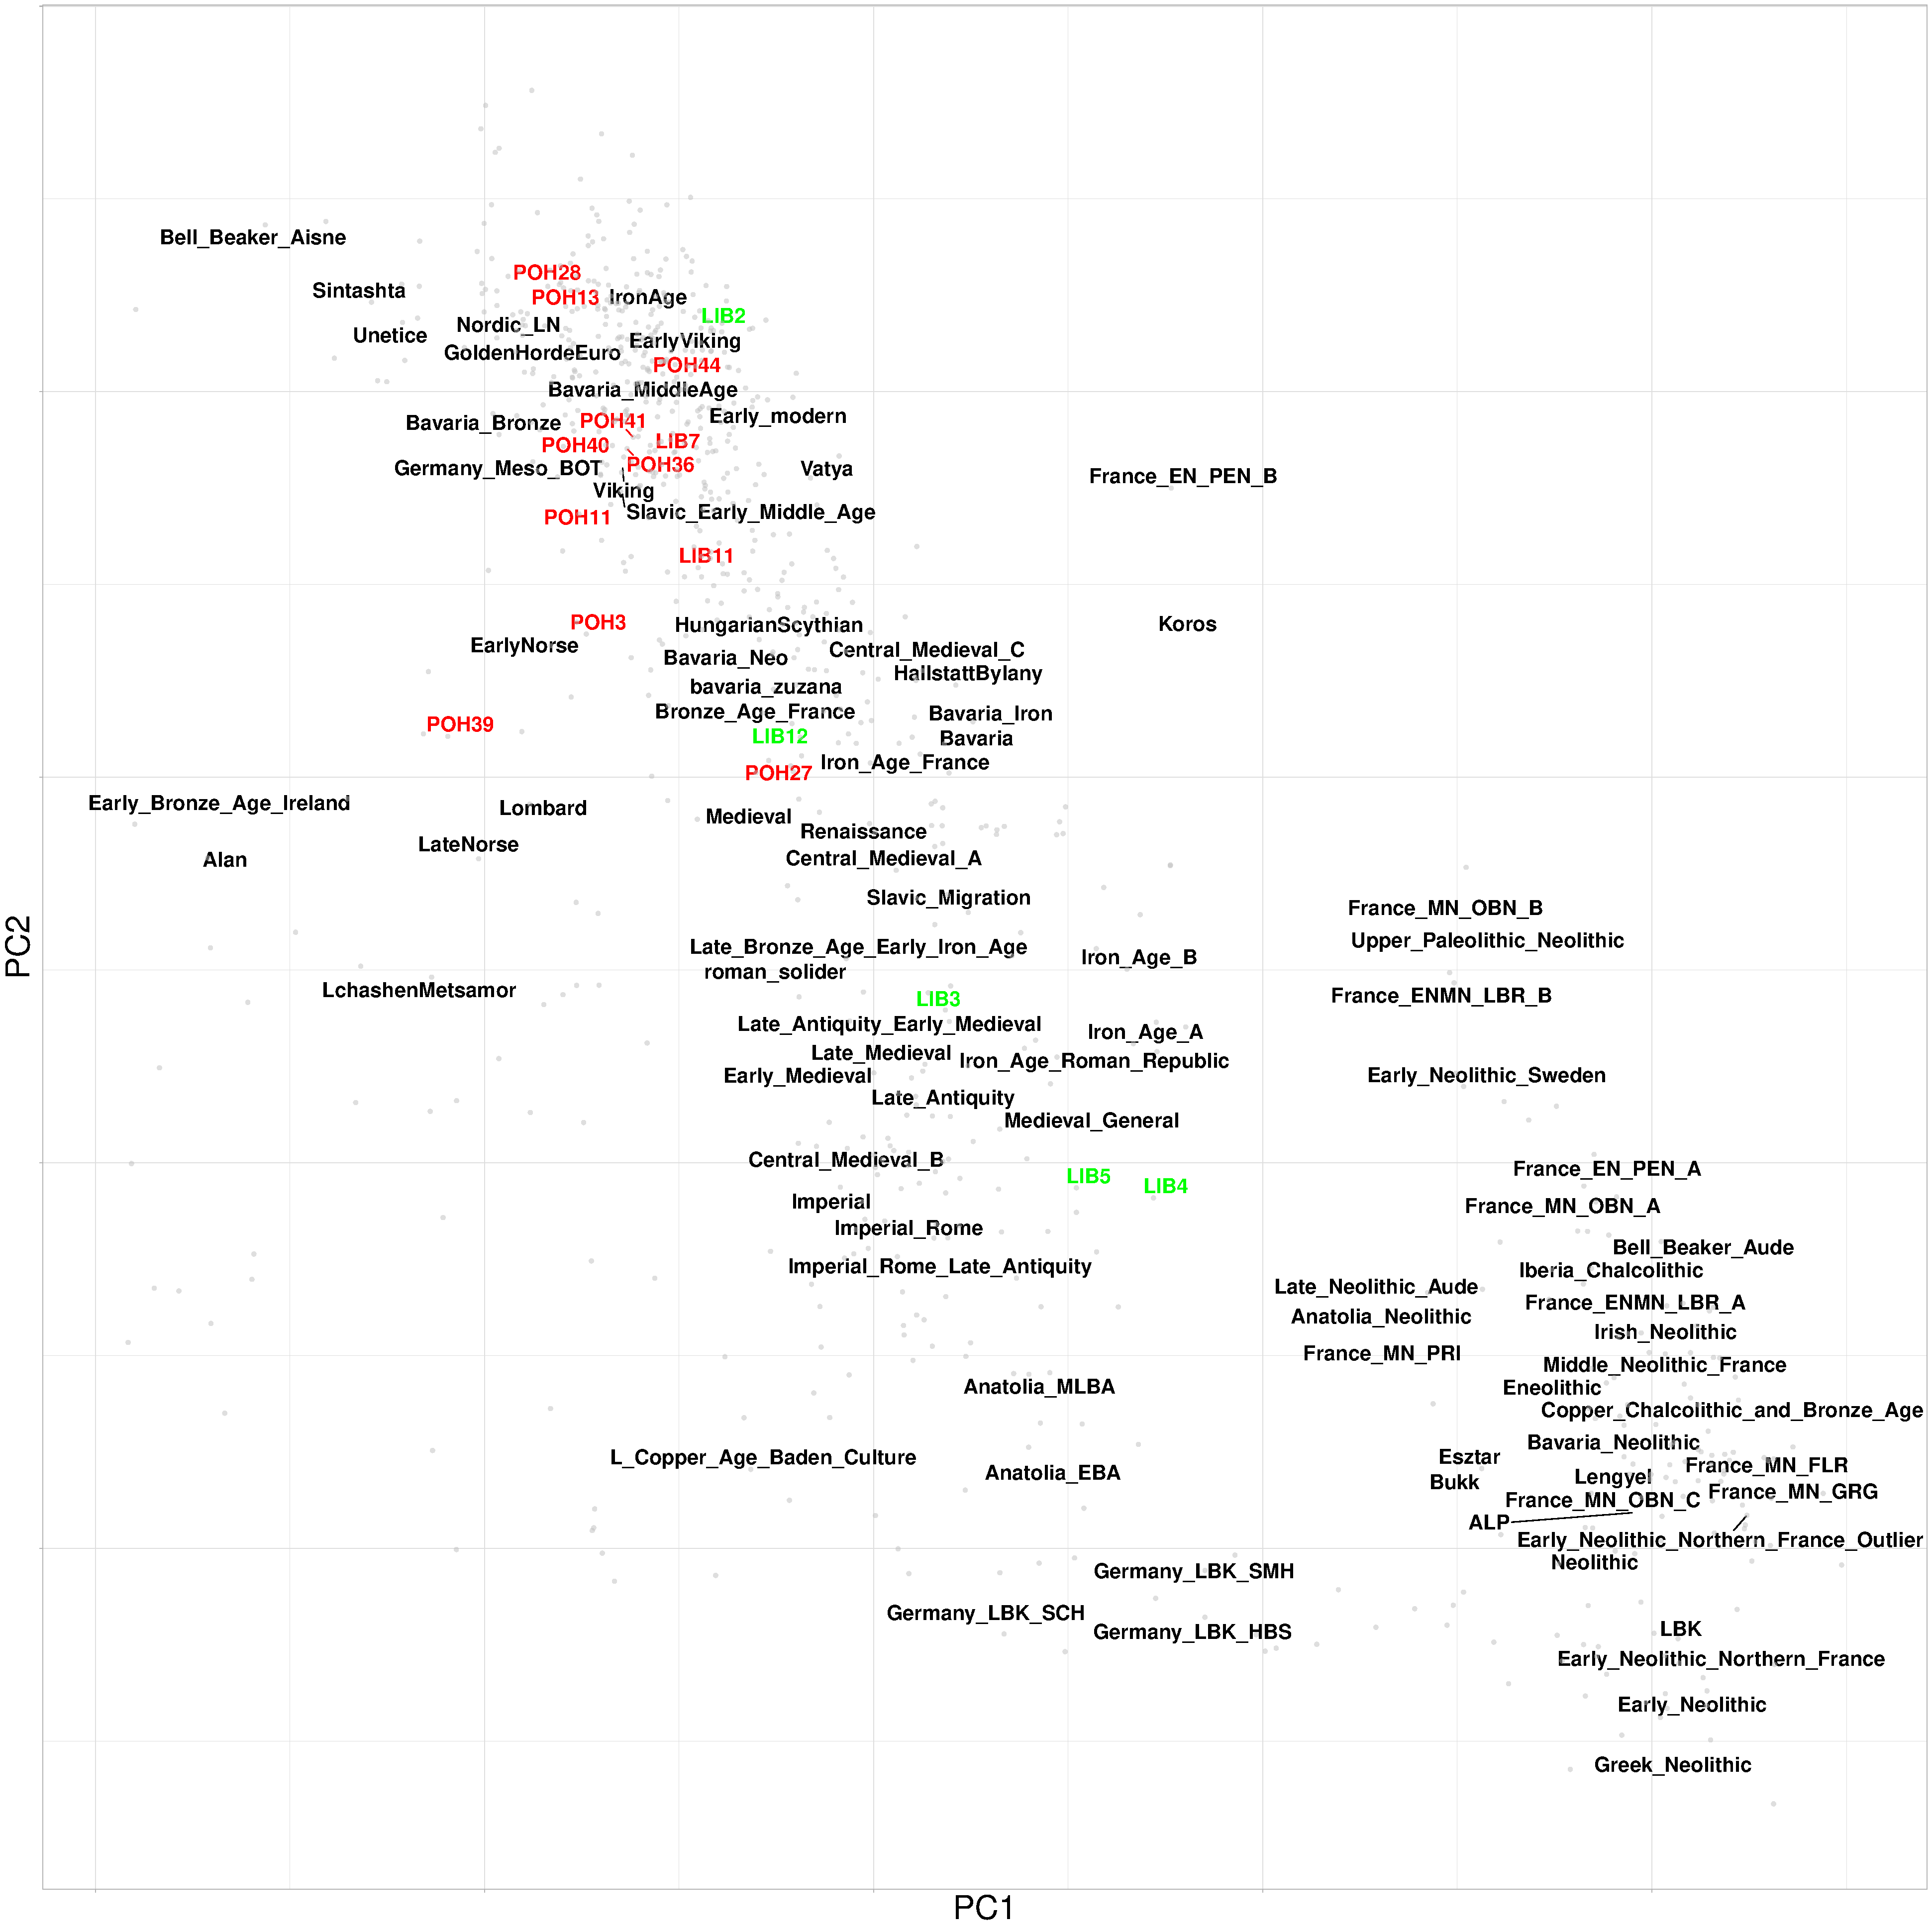
\includegraphics[width=1.0\textwidth]{../images/chapter5/plink_pca.pdf}
    \caption{Principle component plot of newly sequenced ancient samples and reference ancient individuals performed using the plink2. Green labels correspond to Migration Era samples, red labels to Early Middle Age samples and black as reference populations. The position of each reference label is the mean PC coordinates of all individuals within that population}
    \label{fig:AllChr.plink_PCA}
\end{figure}


\subsection{Mixed ancestry of migration period Slavs}

In order to reveal further structure in the ancient samples, I performed an all-v-all painting of 152 ancient samples with a coverage greater than 2x.  I then applied the fineSTRUCTURE clustering algorithm to the samples in order to assign them to genetically homogeneous groups.

The migration period consisted of whole-genomes from 5 individuals from Břeclav (Líbivá), Czech Republic, from 5 different burial sites, who had radiocarbon dates corresponding to the Migration Period (348 - 509AD). It is apparent from both the unlinked (Fig. \ref{fig:AllChr.plink_PCA}) and linked PCAs (Fig. \ref{fig:fs_PCA}) that the Migration Period samples represent a heterogeneous group of individuals who do not originate from the same source population. LIB2 (495AD) is located in the centre of a large cluster of contemporaneous individuals from Iron Age Central and Northern Europe. This individual shares the most haplotypes with Viking individuals from Denmark, Estonia and the UK from roughly the same time period. fineSTRUCTURE analysis grouped LIB2 primarily with Viking era individuals from Sweden, Denmark, Iceland, Estonia and Norway from 300-1100AD. When painted using a present-day set of reference samples, LIB2 matches the most haplotypes and clusters with present-day Norwegians (Fig. \ref{fig:copymatrix_moderns_ancient_slavs}). Put together, these data suggests LIB2 may be a recent migrant from Viking regions. 

\begin{figure}[htp]
    \centering
    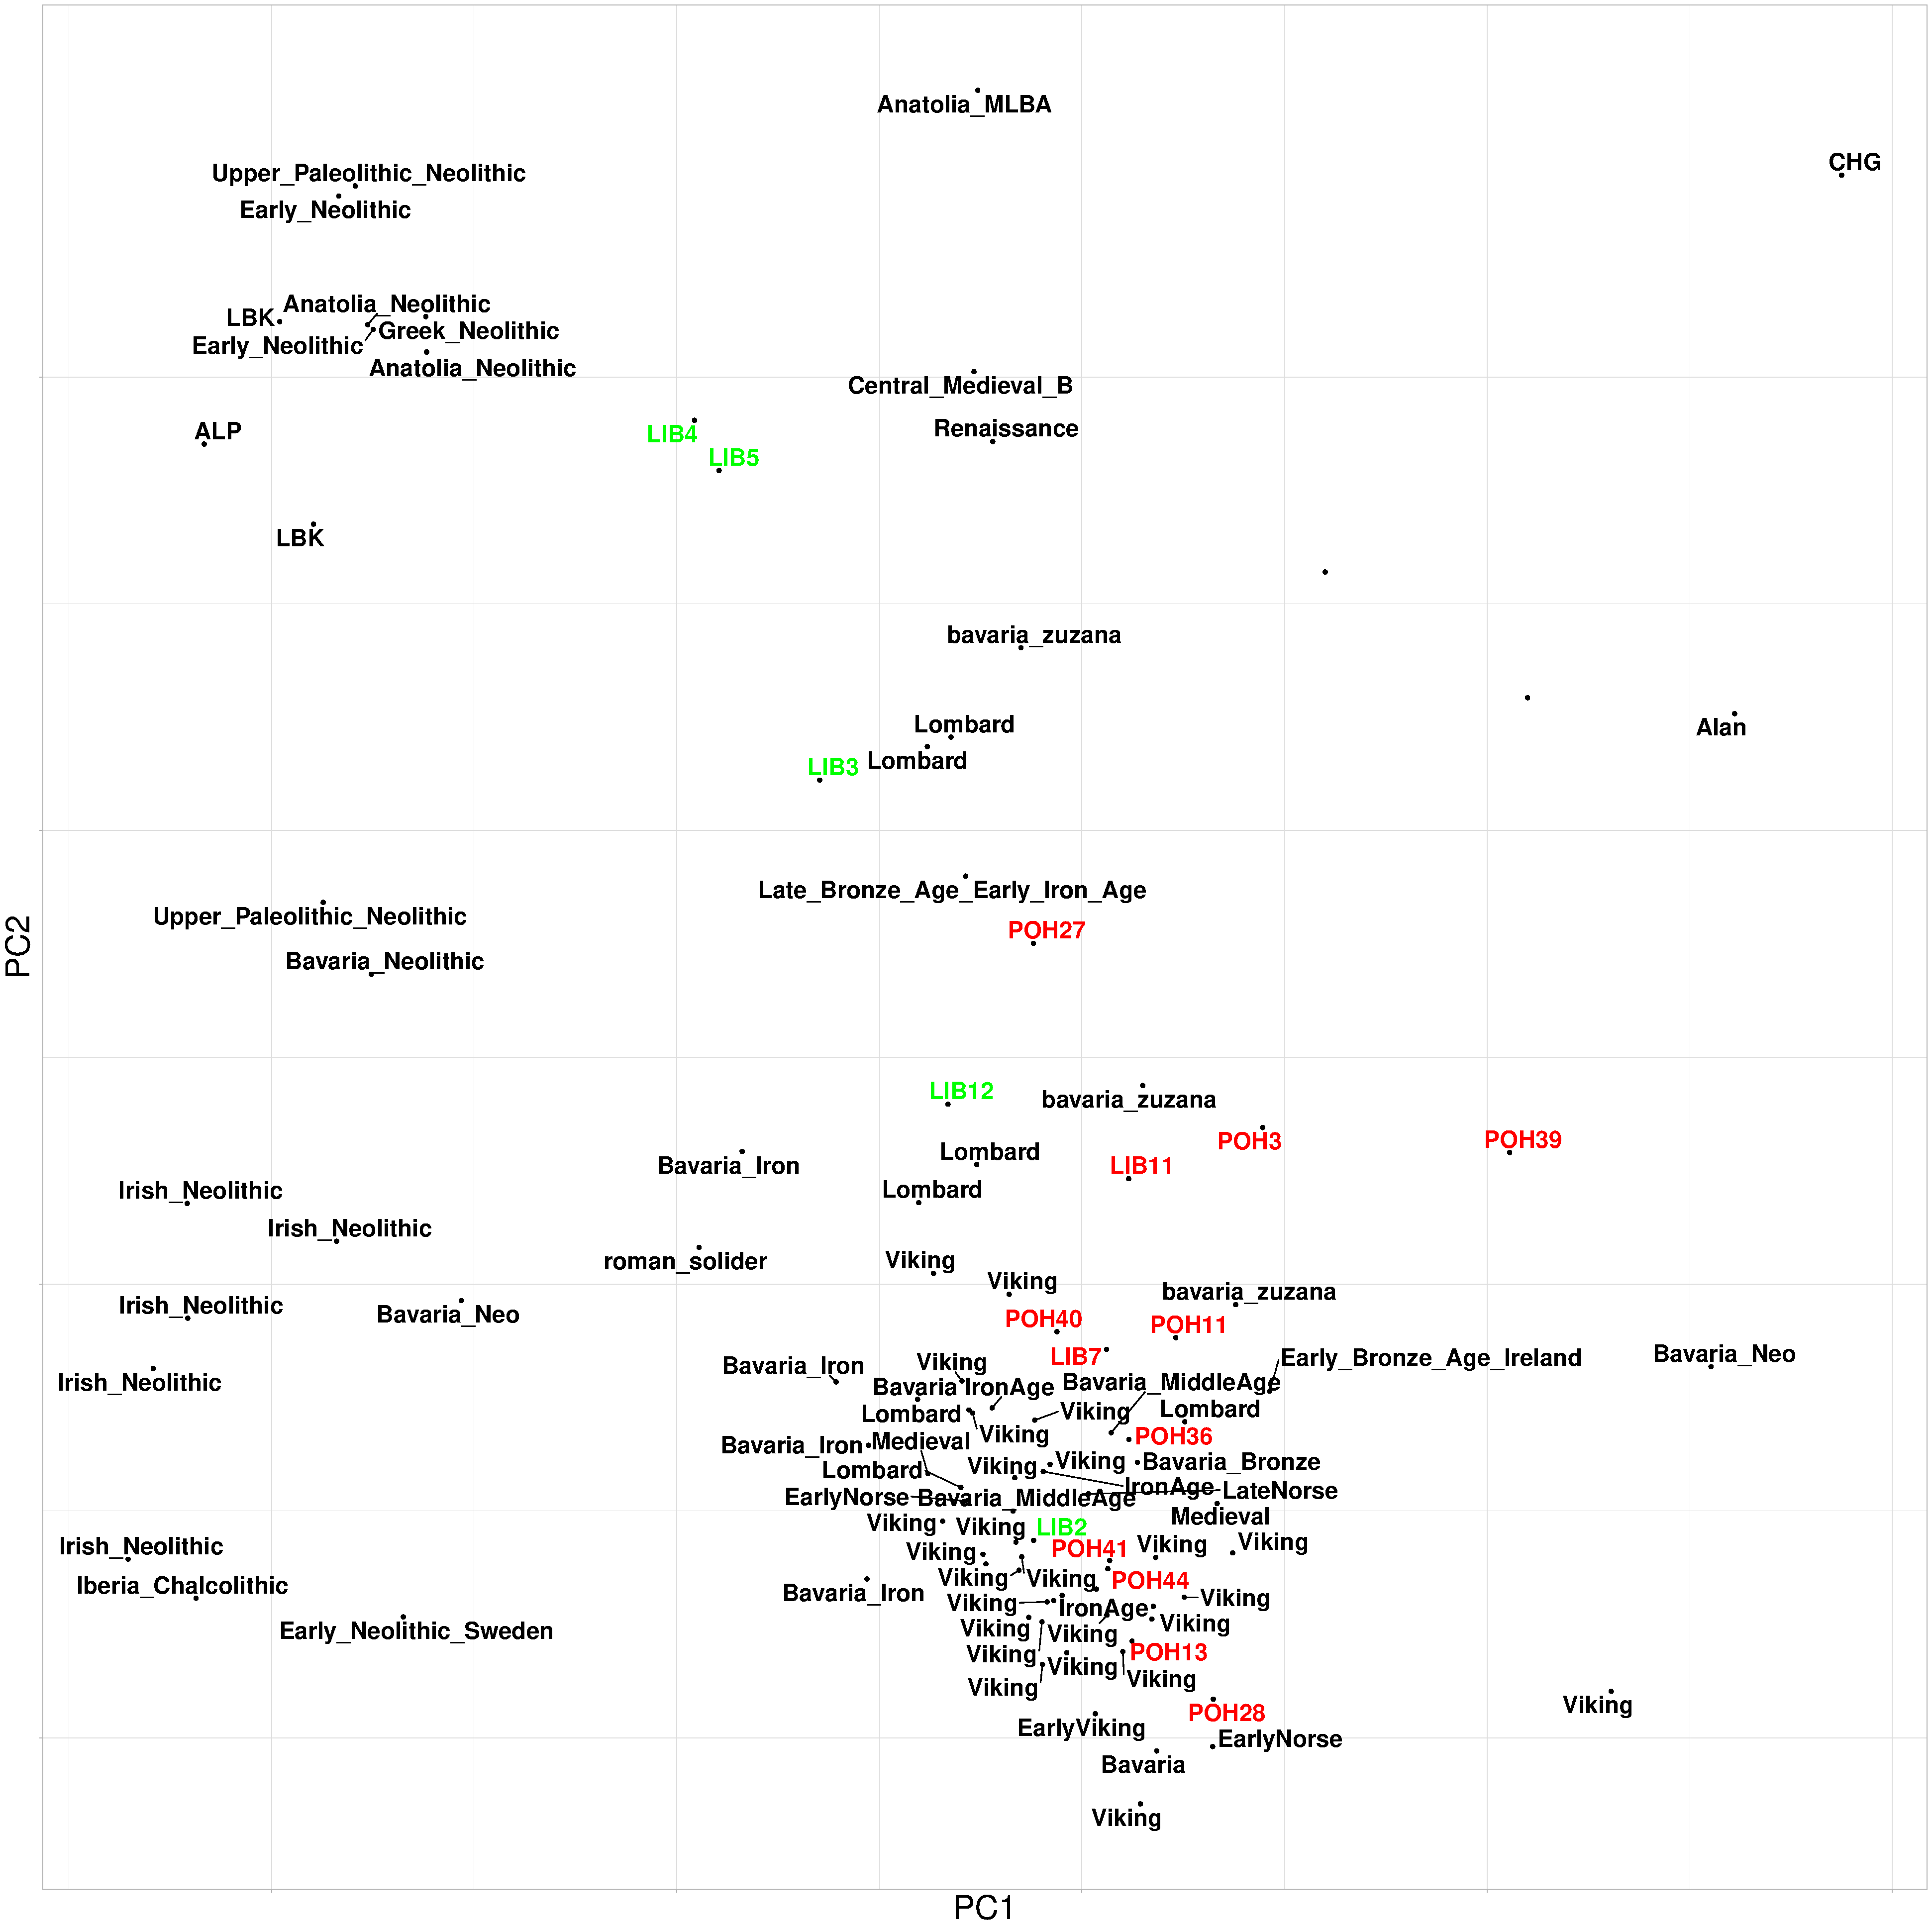
\includegraphics[width=1.0\textwidth]{../images/chapter5/fs_PCA.pdf}
    \caption{Principle component plot of newly sequenced ancient samples and reference ancient individuals performed using fineSTRUCTURE. Green labels correspond to Migration Era samples, red labels to Early Middle Age samples and black as reference populations.}
    \label{fig:fs_PCA}
\end{figure}

There are many sources which detail the links between the Viking and Slavic peoples towards the end of the first millennium \cite{duczko2004viking, peterson2016vikings}. However, most evidence suggests these links occurred later than the date of these samples. For example, it is known that the Scandinavian colonists settled in present-day Russia as early as 750. Therefore, we could suggest that this is evidence of an earlier link than previously known. In their large-scale study of ancient DNA of Viking samples from across Europe, Margaryan et al (2020) present Viking samples and ancestry in Estonia, but not until the beginning of the 8th Century, some 200 years after the estimated date of LIB2.  

On the other hand, LIB4 and LIB5, show an affinity the European Neolithic, indicated by their position on the linked and unlinked PCA. Interestingly, they share the most haplotypes with several Italian Neolithic samples, despite being separated by approximately 6000 years (not a clue why this is). Despite sharing the most haplotypes with these samples, LIB4 and LIB5 are found in fineSTRUCTURE clusters with more recent samples from Italy (Early Iron Age / Renaissance), suggesting the link to Neolithic Italy may have been transmitted by more recent populations (need to expand more on this). Both LIB4 and LIB5 share the most haplotypes with one another; this and their consistent positions on PCA and fineSTRUCTURE groupings suggest they are closely related and could be from the same local population. 

The appearance of Neolithic-like ancestry deep into the first millennium is similar to a signal found in a study exploring the ancestry of individuals with elongated skulls in medieval Bavaria (approximately 500AD) \cite{Veeramah2018}, where it was discovered particular individuals harbour substantial `southern' ancestry from outside of Bavaria, closest to individuals from present-day Greece and Turkey. There are at least two possible explanations for the presence of this ancestry in the Migration Era samples. Firstly, LIB3, LIB4 and LIB5 may be similar migrants to the region. This is consistent with the fact that (at least LIB3, need to check others) is female; Veeramah et al (2018) showed that there was a tendency for females to migrate from southern regions, perhaps related to the formation of strategic alliances. Alternatively, it is possible these individuals are a leftover from a historically described Lombard migration that moved from Northern Germany (nobody really knows where it started according to Zuzana) through Czechia, Slovakia, Hungary and ended up in Lombardia. Accordingly, this could appear as genetic similarity to present-day populations from Northern Italy. This hypothesis is supported by the clustering of LIB3, LIB4 and LIB5 with present-day Italian samples in the `present-day' fineSTRUCTURE analysis (Fig \ref{fig:tree_with_ancients}).

Ancestry proportion estimation using SOURCEFIND showed that the cluster containing these samples shares 25\% of their ancestry most recently with people from Anatolia, 16\% from LBK (Linearbandkeramik) and 12\% from a cluster containing Lombard individuals. 

I performed MOSAIC admixture modeling using present-day samples as surrogates and the clusters of newly sequenced ancient samples as targets. I did not detect an admixture even when targeting LIB3, LIB4 and LIB5. This could be due to low power or a low number of samples, or that the samples are unadmixed with respect to the surrogate populations.

On the fineSTRUCTURE PCA, LIB3 clusters with Lombard samples from Northern Italy. Historical evidence cites alliances between Slavs and Lombards in the 5th century \cite{lotter2003volkerverschiebungen}. In the `present-day' painting, LIB3 clusters with and shares the most haplotypes with present-day Tuscans.  

Finally, LIB12 displays ancestry which is more typical of the preceding Central European Bronze Age. It copies the most haplotypes from samples from Bronze Age Ireland (Rathlin) and Bavaria and is found in a cluster with several other Bronze Age samples. This suggests it may represent a `leftover' from a local Bronze Age population which was unaffected by the Antiquty / Iron Age migrations to the region.

\subsection{Early Middle Age Slavs}

In comparison to the 5 Migration Period ancient Slavs, the 12 Early Middle Age Slavs (741-956 AD) represent a more homogeneous set of samples. All 12 samples were clustered into the same fineSTRUCTURE group (named Slavic Early Middle Age II), alongside Viking/Medieval samples from Ukraine, Poland and Sweden. SOURCEFIND analysis showed that this cluster derives roughly equal parts of ancestry from the clusters  Viking 10C Scan I, BronzeAge I and Lombard mixed cluster. Interestingly, these are 3 ancestry sources which are similar to those found in the Migration Period samples. We could tentatively therefore suggest that the Early Middle Age Slavs were formed from the mixture of `Northern' (represented by Viking) and `Southern' represented by Lombard onto a substrate of local Bronze Age populations. Note that I suggest that these are the most representative populations and not necessarily the `true' populations that mixed.

MOSAIC admixture modeling using ancient surrogates proved inconclusive. However, using present-day individuals as surrogates provided cleaner results. The best fitting model was a 3-way admixture event involving sources closest to present-day day North-Central Slavs (76.6\%), Southern-Eastern Slavs (21.9\%) and East Asians, best represented by Mongolians (1.5\%) (Fig. \ref{fig:EarlyMiddleAges_MOSAIC_3way_moderns_Mu}. This admixture even was estimated to have occurred 9.4 (2.5\% 5.7gens - 97.5\% 17.9gens) generations before the samples (Fig. \ref{fig:EarlyMiddleAges_AdmixtureProportionsPlot}). 

This admixture event is consistent with a signal found in both present-day day Eastern European individuals \cite{MOSAIC_2019, Hellenthal2014}. In previous studies, this admixture event was dated to approximately 1200CE (MOSAIC) and 438CE (GLOBETROTTER). Despite the differing dates, the proportion of ancestry is consistent across studies (approximately 2\%), suggesting the signal is genuine. To further support the event, the proportion of ancestry from this source is consistent across 2-way and 3-way MOSAIC admixture models. 

\begin{figure}[htp]
    \centering
    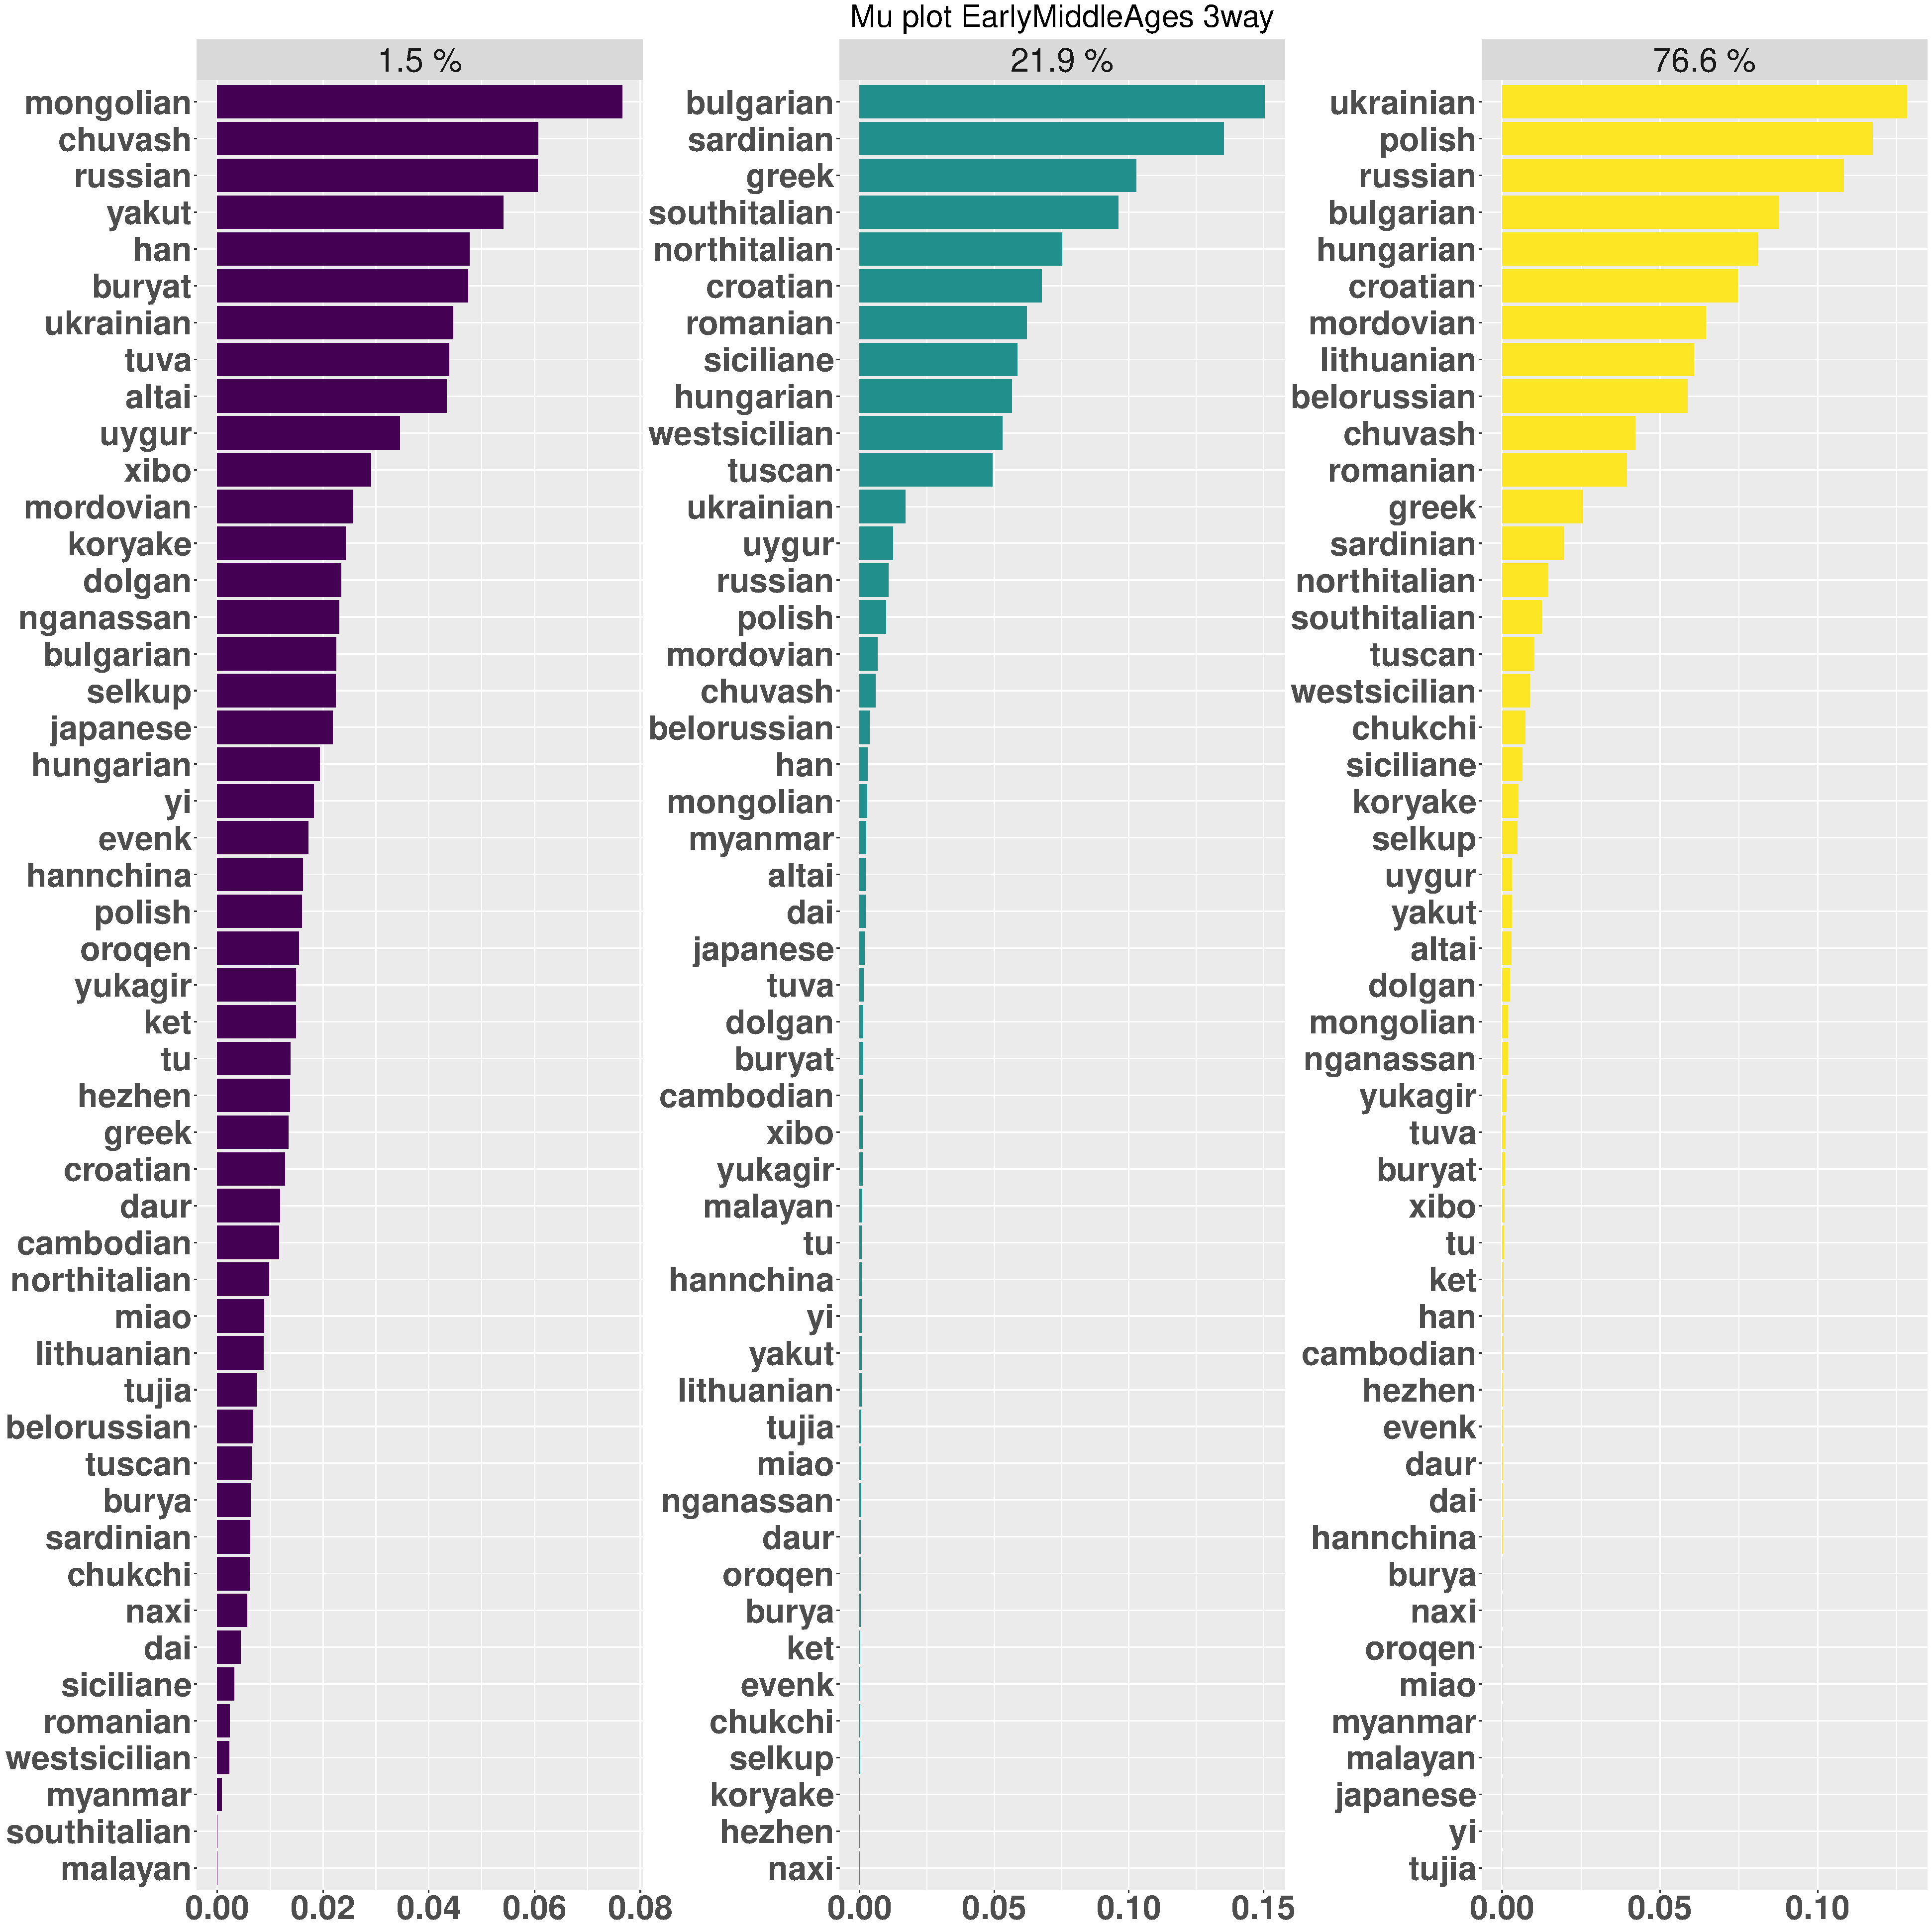
\includegraphics[width=1.0\textwidth]{../images/chapter5/Mu_plot_EarlyMiddleAges_3way.pdf}
    \caption{Copying matrix plot for sources in 3-way admixture event for Early Middle Age ancient Slavic samples. Each panel represents one of the 3 putative mixing sources. Labels above each panel gives the proportion that mixing source contributed to the Early Middle Age samples. Length of the bars within each panel represent the amount that putative mixing source copied from a particular population.}
    \label{fig:EarlyMiddleAges_MOSAIC_3way_moderns_Mu}
\end{figure}

\begin{figure}[htp]
    \centering
    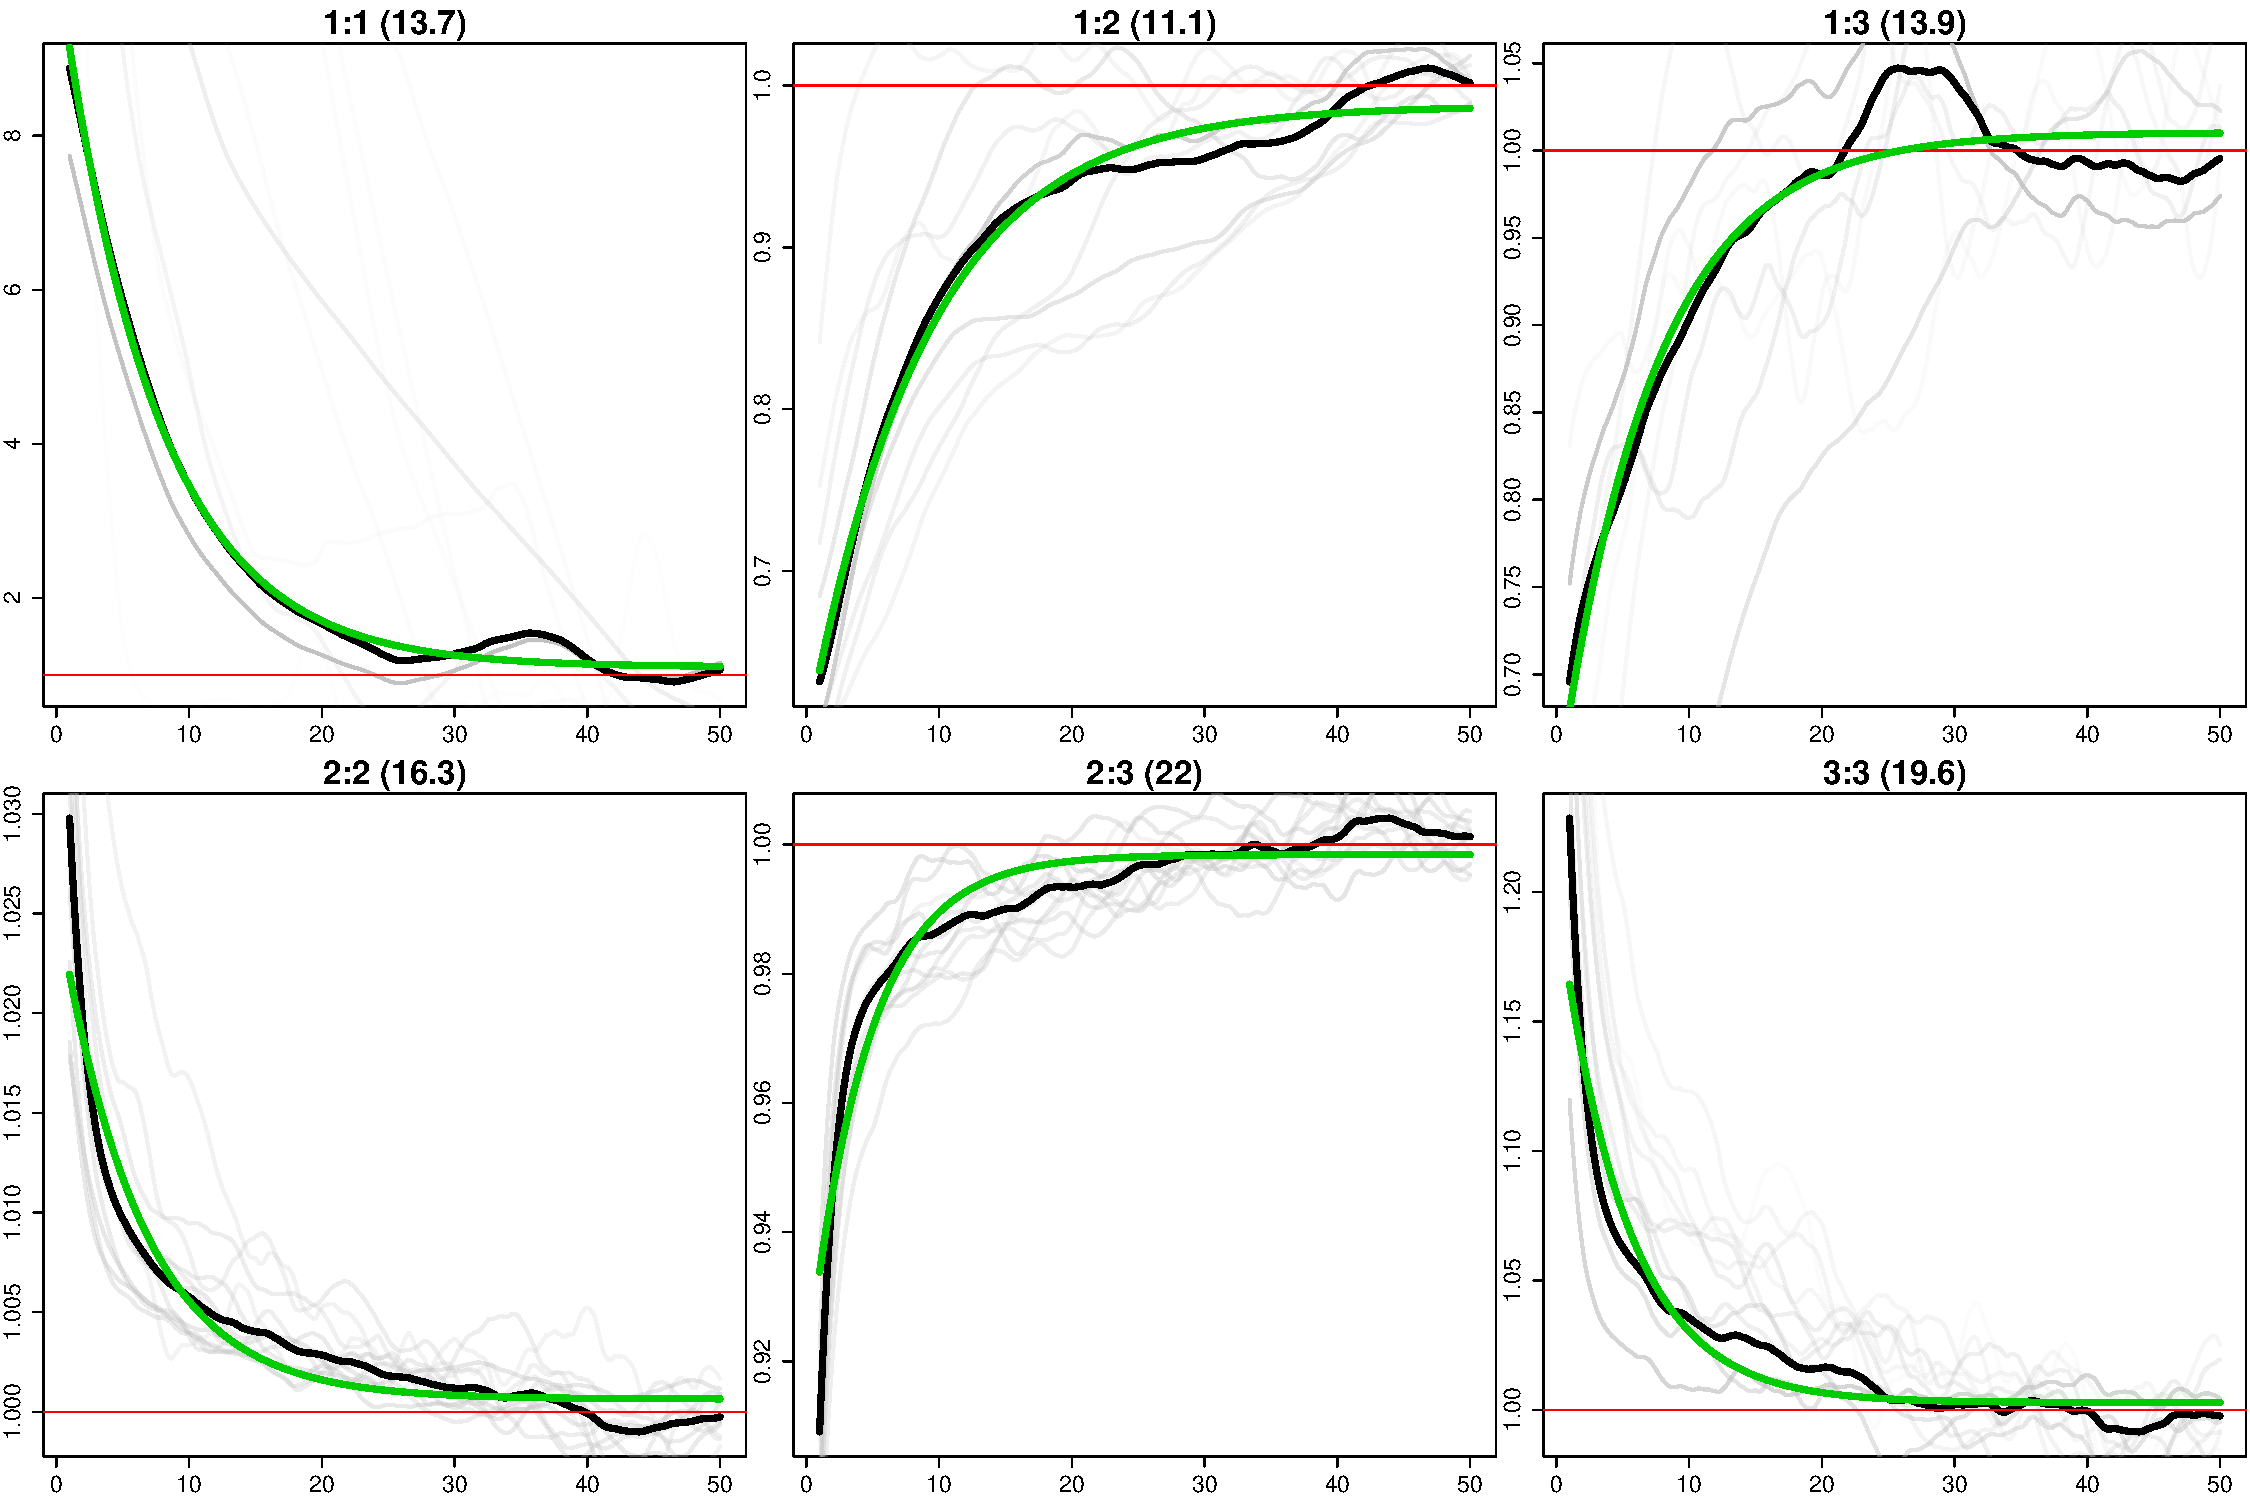
\includegraphics[width=1.0\textwidth]{../images/chapter5/EarlyMiddleAges_3way_acoanc.pdf}
    \caption{Inferred Coancestry Curves obtained from modeling Early Middle Age samples as a 3-way mixture of present-day individuals. Black lines are empirical coancestry curves across all target individuals, light grey are per individual, green is the fitted single-event coancestry curve. Note to self - need to figure out what the numbers mean but doesn't say in the manual anywhere.}
    \label{fig:EarlyMiddleAges_MOSAIC_3way_moderns_acoanc}
\end{figure}

\begin{figure}[htp]
    \centering
    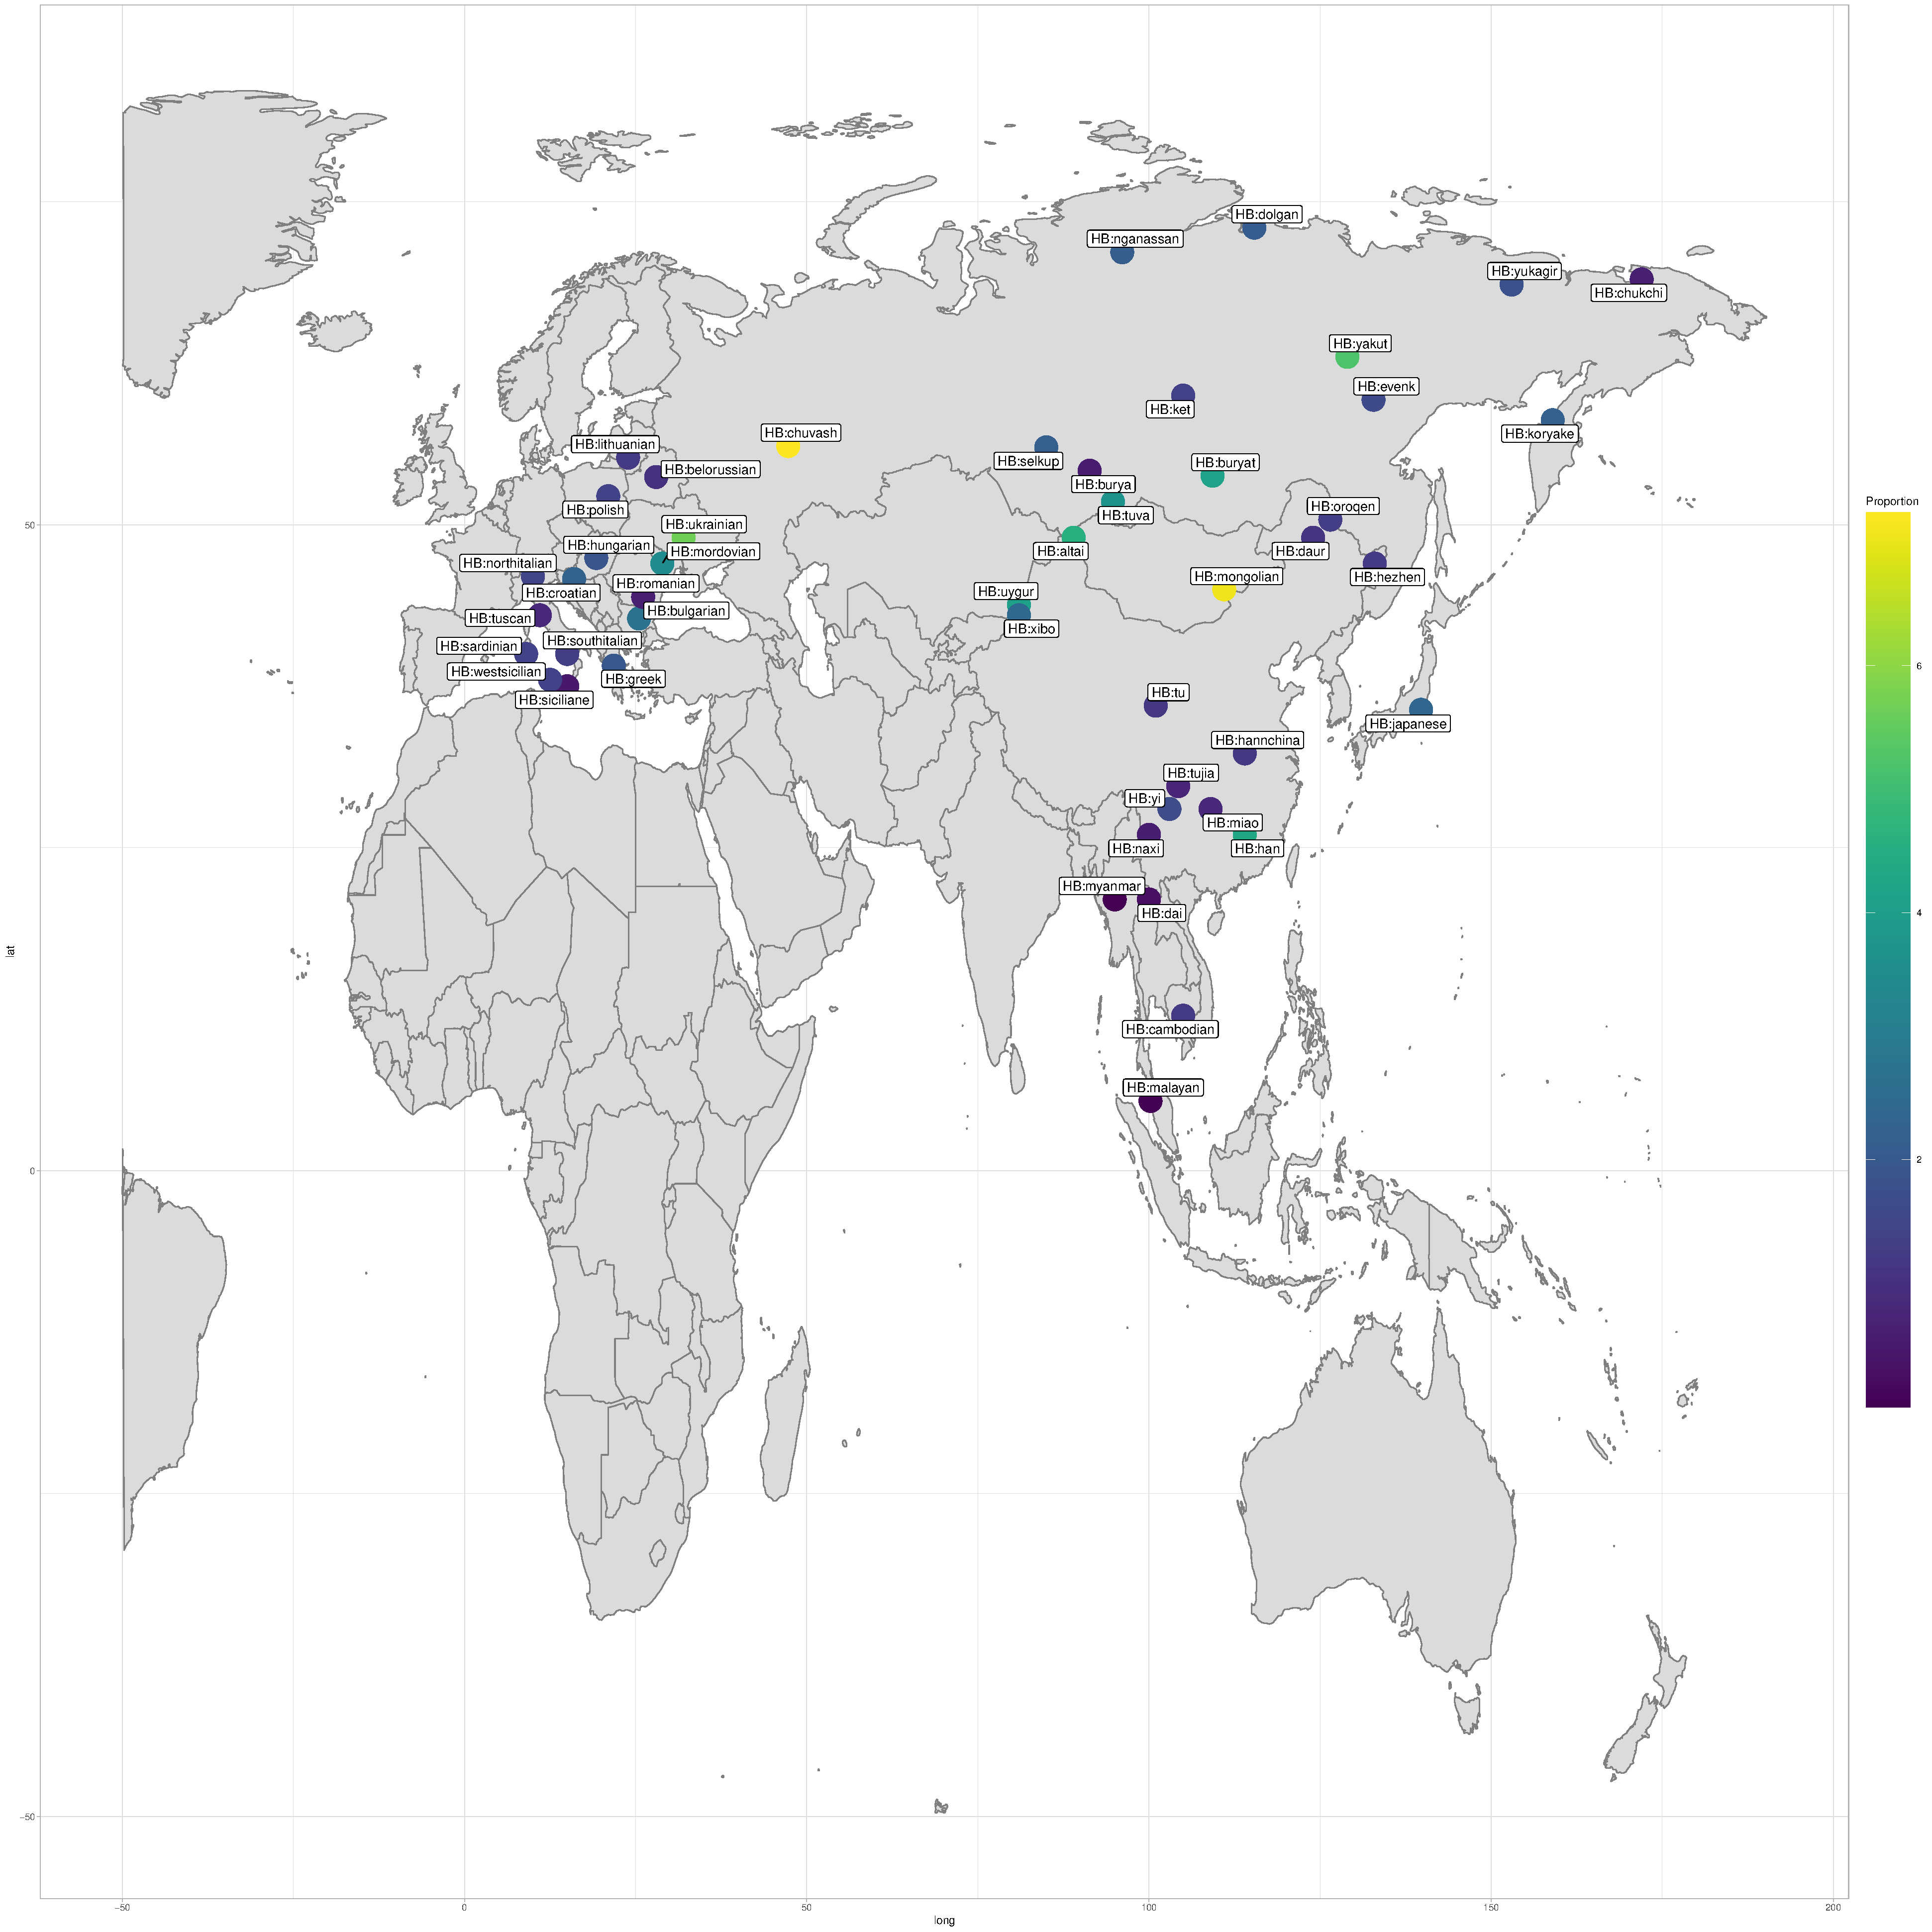
\includegraphics[width=1.0\textwidth]{../images/chapter5/EarlyMiddleAges_AdmixtureProportionsPlot.pdf}
    \caption{Distribution of East-Asian minor ancestry component in Early Middle Age samples.}
    \label{fig:EarlyMiddleAges_AdmixtureProportionsPlot}
\end{figure}

\subsection{Do the samples cluster together - TVD permutation test}

fineSTRUCTURE analysis suggested that the Migration Era and Early Middle Age samples did not originate from the same source population. To formally establish whether the Early Middle Age and Migration Period samples cluster within their respective populations, following Leslie et al 2015 \cite{Leslie2015}, ,I performed a TVD permutation test. TVD is a distance metric which can be calculated from the chunklengths matrix and is equivalent to finding the absolute distance between two copyvectors, with larger values meaning two samples have more different ancestry profiles.

Using the ancients chunklengths matrix, I grouped the samples into Migration Period and Early Middle Age and  calculated the average copyvectors $C_{mp}$ and $C_{ema}$ across samples within each groups. Then, I calculated the empirical TVD between the two groups as $TVD_{mp,ema} = \sum |C_{mp} - C_{ema}|$. For 10,000 iterations, I then randomly permuted the population labels among the samples and then calculated a `random' TVD, $TVD_{mp,ema}^{rand}$ between the samples with randomly permuted populations. We can then calculate the p-value that we can reject the null model of no significant differences between the groups (not sure if this is the right way of wording it) as the number of randomly permuted iterations where $TVD_{mp,ema}^{rand} > $ $TVD_{mp,ema}$. This test supported clustering the samples into their respective groups ($p=0.0013$).

This is in agreement with the fineSTRUCTURE results which grouped together all of the Early Middle Age samples together to the exclusion of the Migration Period samples. 

\subsection{Interactions between the two groups}

The previous section suggested that individuals from the Migration Period and Early Middle Ages had differing ancestry signals. 

To determine the extend of mixture and continuity between the Migration Period and Early Middle Ages, I modeled each Early Middle Ages sample as a mixture of other ancients, including individuals from the preceding Migration Period. The proportion of ancestry the individuals derive from the Migration Period clusters could be used as a proxy for the degree of continuity. The proportion of ancestry derived from the Migration Period was low (mean 3.4\% , range 0.4\% - 12.5\%), suggesting that there was a relatively large scale population replacement between the two different time periods. 

Note - I could do something like admixture f3 to see if Early Middle Age is admixed between Middle Age and any other pop instead as a more explicit test.

\subsection{Legacy of Slavic migrations in present-day individuals}

To understand the genetic legacy the newly sequenced Slavic samples left in different European populations, I painted each sample using the HellBus dataset of present-day individuals. This dataset contains a diverse set of European populations - particularly those from present-day Slavic speaking countries (Polish, Croatian, Bulgarian, Belorussian, Ukrainian, Russian) but also neighbouring non-Slavic speaking countries (Romanian, Lithuanian, Germany and Mordovia).  

Principle component analysis (PCA) of the chunklengths matrix, where present-day European samples acted as donors, reveals genetic similarity between ancient Slavic samples from the Early Middle Ages and present-day day Slavic speaking people (Fig. \ref{fig:chunklengths_moderns_ancients_PCA}). The samples primarily cluster with present-day Polish and Belorussian individuals, but appear to fall on a cline of genetic similarity between Russians and Southern Europeans. This cline could be mediated by the possible historical admixture event between a source closest to present-day East Asians and a second closest present-day Southern Europeans, with the position of the samples along the cline dependent on the level of admixture from the different sources.

As with previous analyses, Migration Era Slavs are spread across the PCA. 3 samples, LIB3, LIB4, and LIB5 cluster with present-day Italians, consistent with deriving a substantial ancestry component from Neolithic-like sources. LIB4 and LIB5 appear to be positioned closer to Southern Italians and Greeks, whereas LIB3 is closer to Northern Italian and Tuscan populations. 

LIB2 shows a strong affinity to present-day Norwegians, suggesting it may be a recent migrant from Viking regions. 

\begin{figure}[htp]
    \centering
    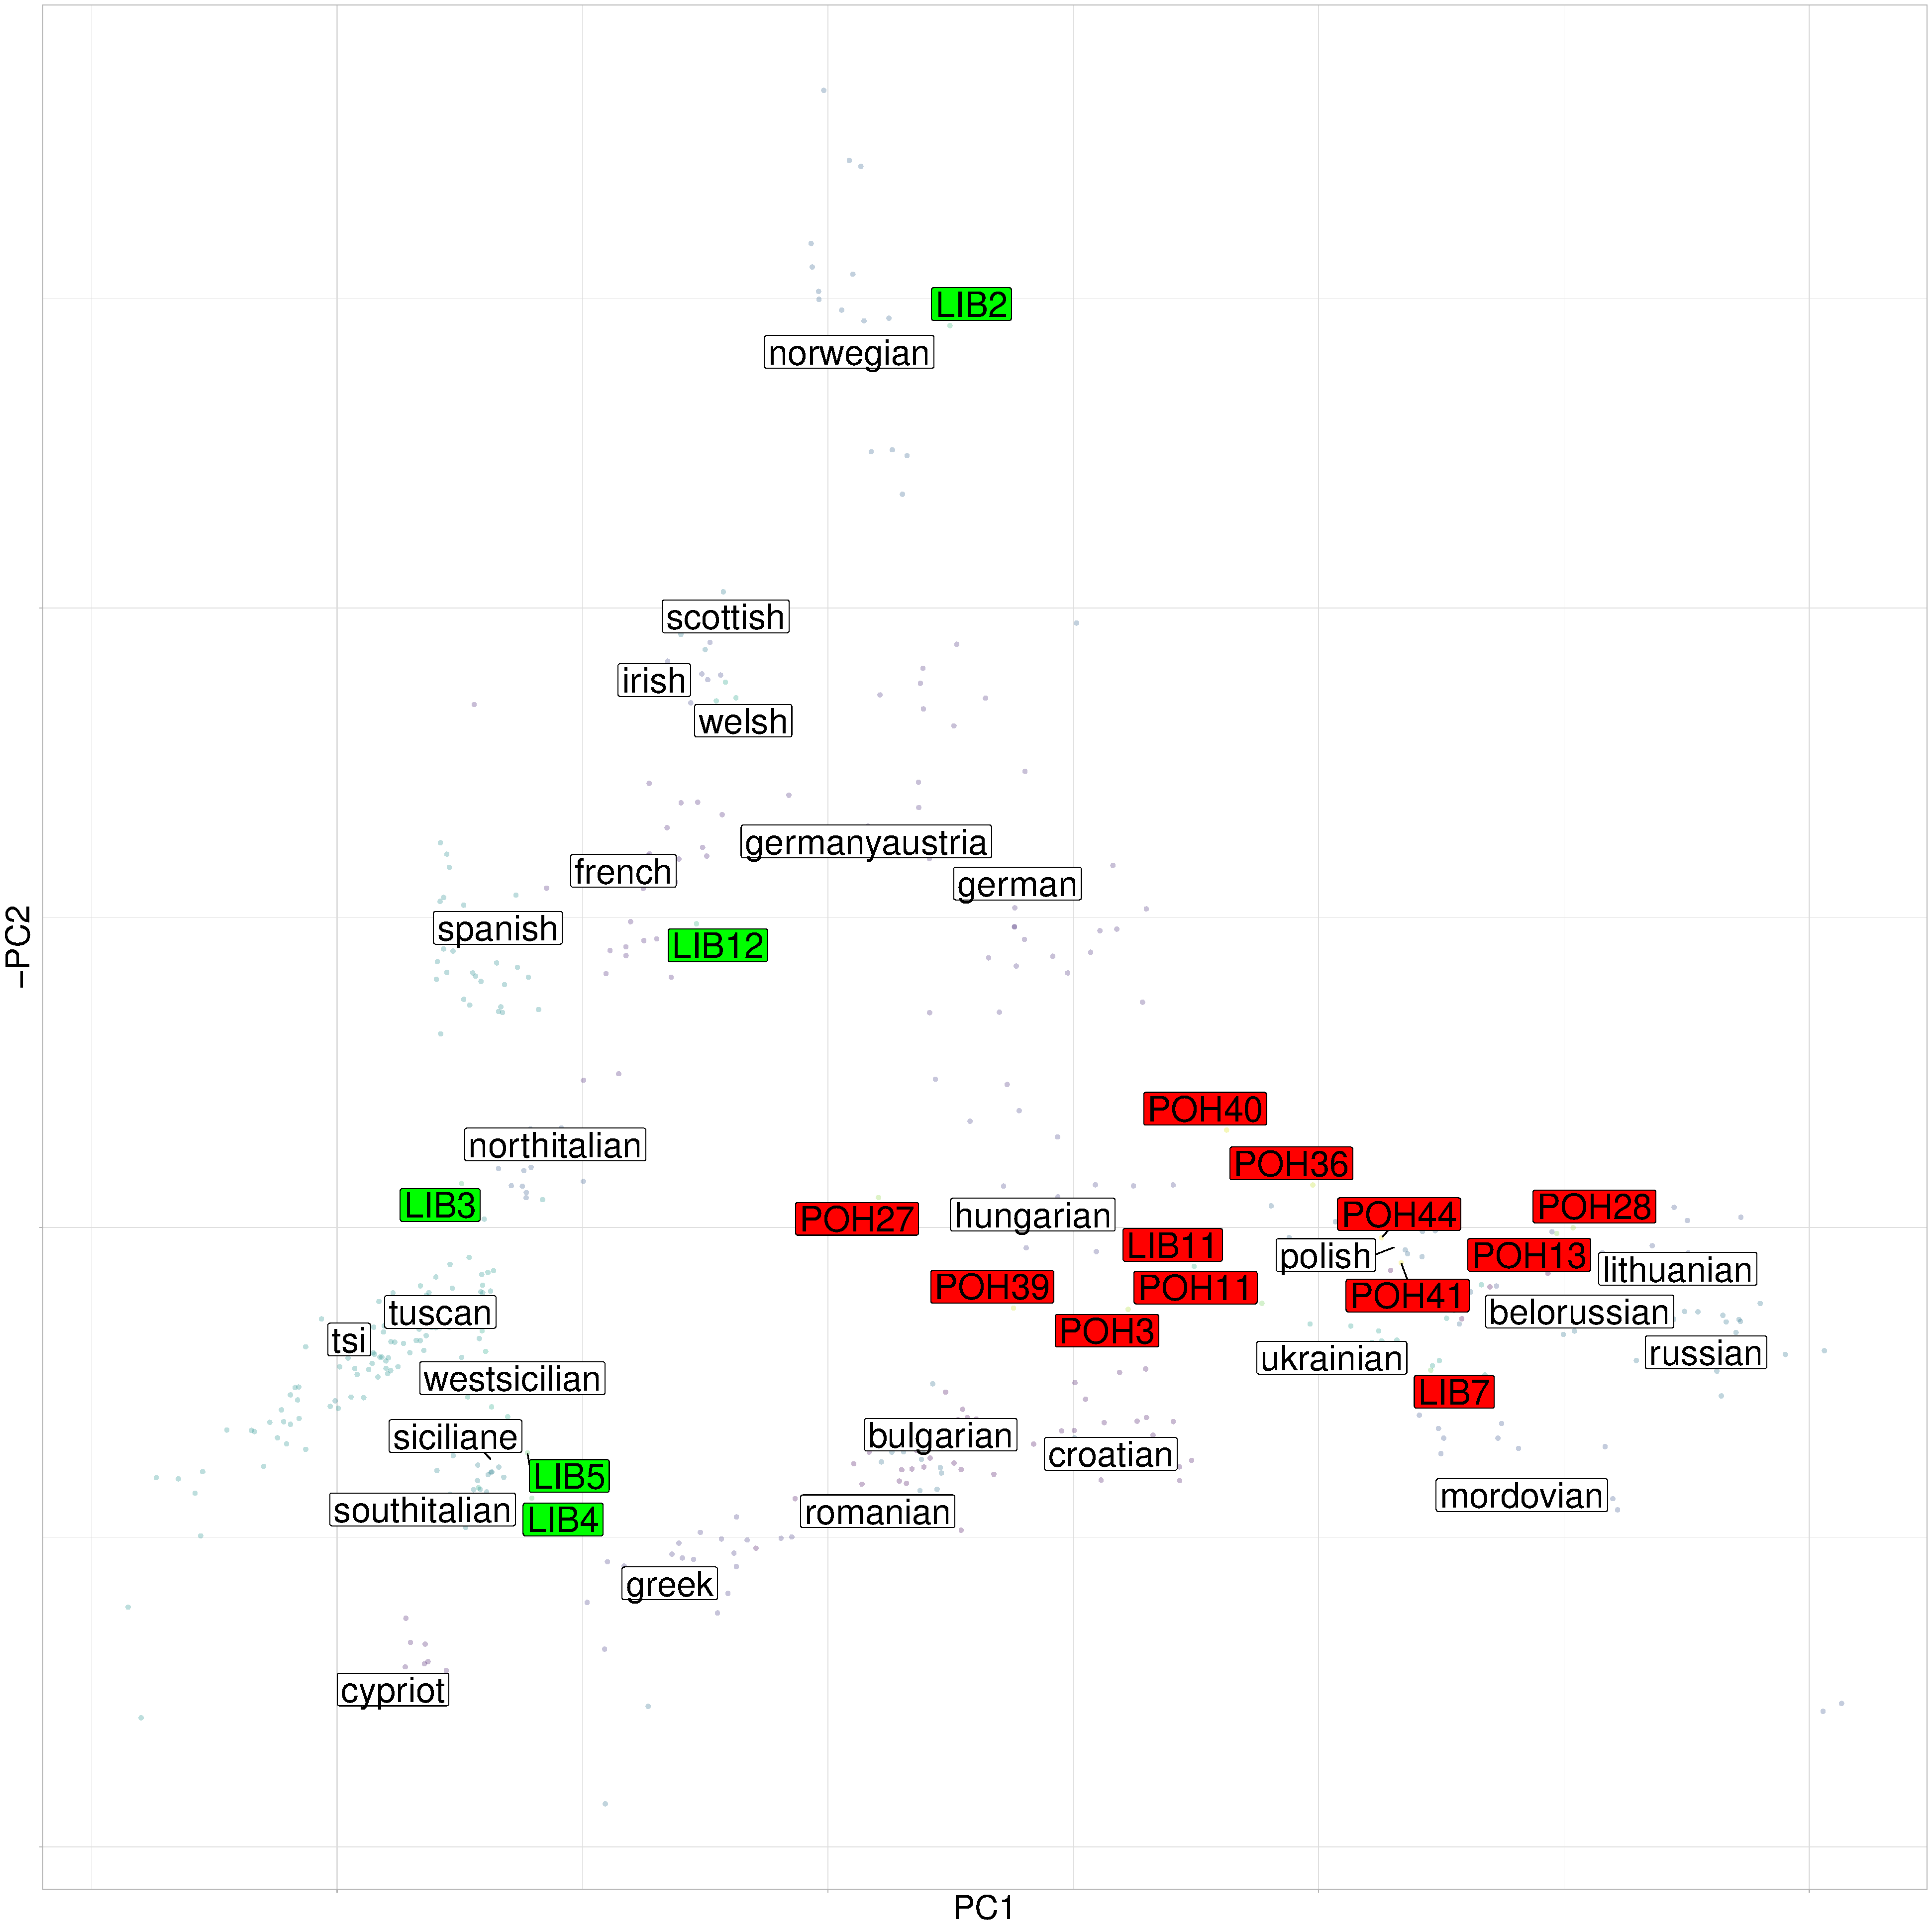
\includegraphics[width=1.0\textwidth]{../images/chapter5/chunklengths_moderns_ancients_PCA.pdf}
    \caption{Principle component plot of newly sequenced ancient samples and reference modern individuals performed using the finestructure library. Green labels correspond to Migration Era samples, red labels correspond to Early Middle Age samples and white labels correspond to reference populations. The position of each reference label is the mean PC coordinates of all individuals within that population. Transparent coloured points correspond to present-day individuals.}
    \label{fig:chunklengths_moderns_ancients_PCA}
\end{figure}

The same pattern can be observed on the raw copyvector output matrix (Fig. \ref{fig:copymatrix_moderns_ancient_slavs}). The Migration Era samples appear not to show any excess affinity to present-day day Slavic populations. The two samples who in previous analysis showed a strong genetic relationship to the Neolithic, LIB4 and LIB5, shared the most haplotypes with present-day day Greek individuals. This should not be surprising given present-day day Greeks have a relatively high proportion of Neolithic ancestry relative to other European populations \cite{lazaridis2017genetic}. 

\begin{figure}[htp]
    \centering
    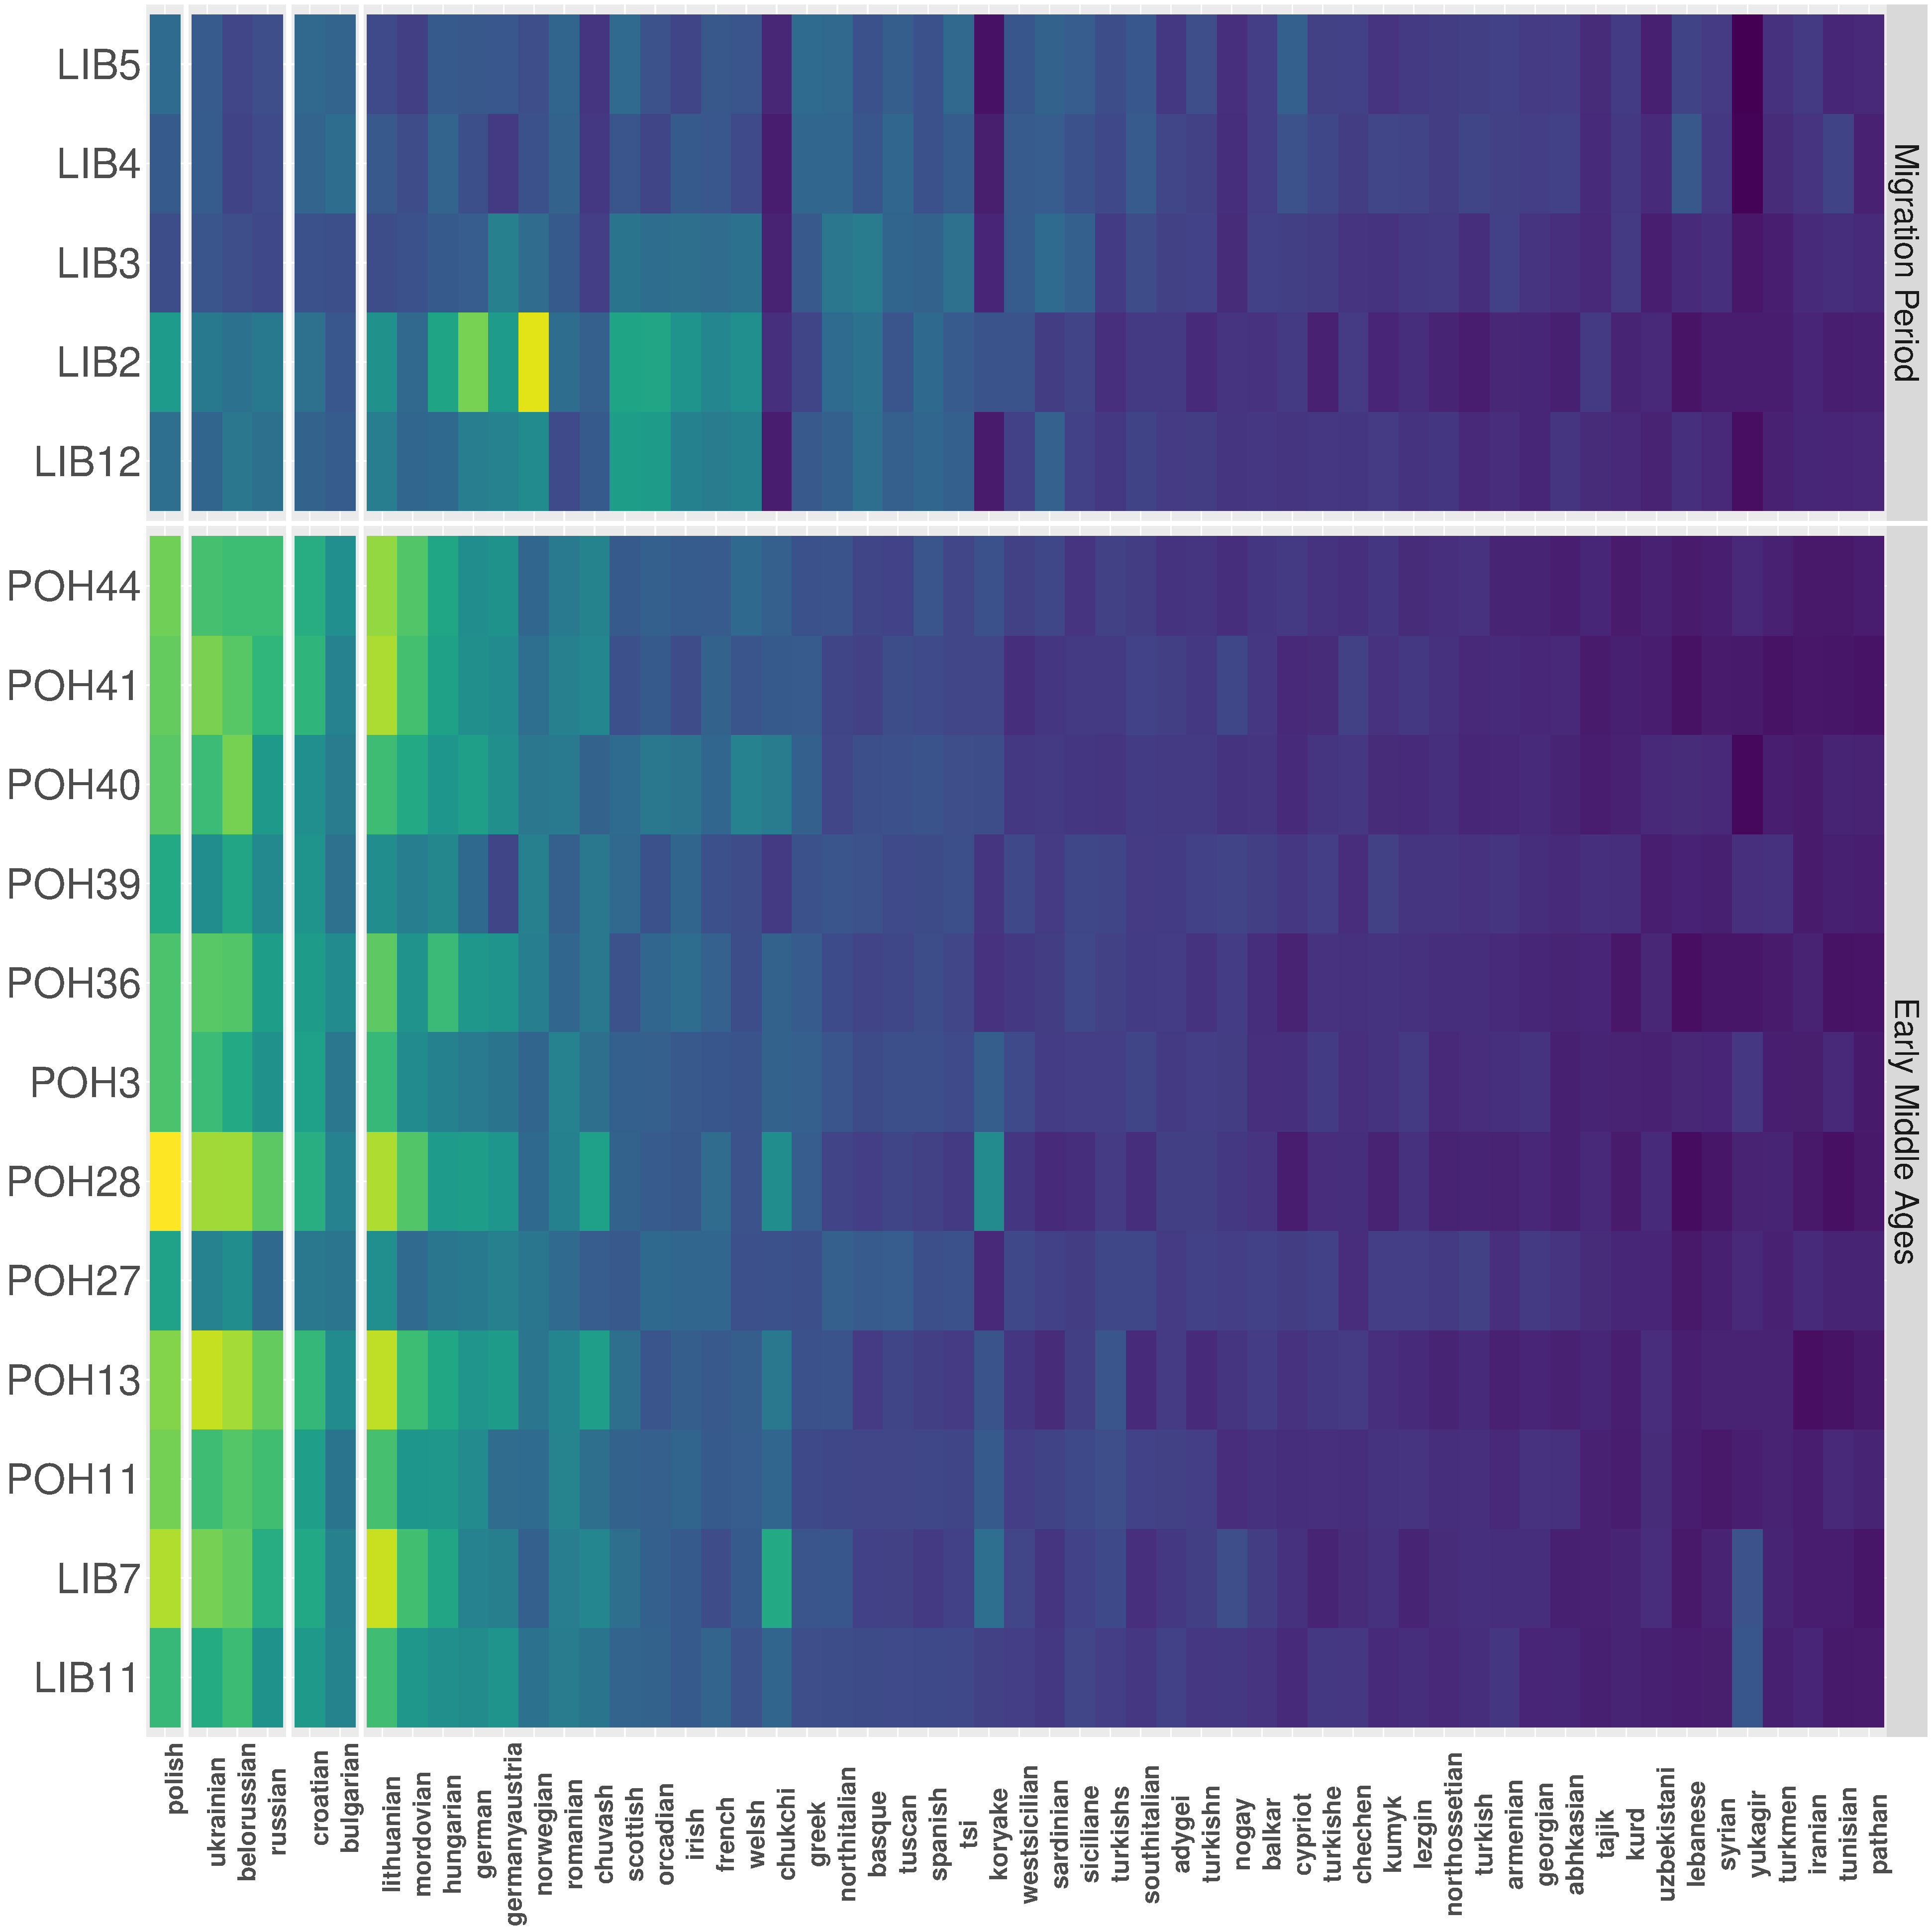
\includegraphics[width=1.0\textwidth]{../images/chapter5/copymatrix_moderns_ancient_slavs.pdf}
    \caption{Raw chunklengths matrix from the `present-day' painting. Rows correspond to different ancient recipient individuals, grouped into Migration Period and Early Middle Age period, and columns to different donor populations. Colour of cells corresponds to the total length of genome that a given donor individuals donates to that recipient, with dark/blue  indicating less sharing and light/yellow colours indicating more sharing.}
    \label{fig:copymatrix_moderns_ancient_slavs}
\end{figure} 

In contrast, the Early Middle Age samples showed a strong affinity to present-day day Slavic populations. In particular, we find that samples copy many more haplotypes from present-day day Polish individuals than they do from other populations. This is consistent with previous findings based on uniparental markers. There was also a strong affinity to several non-Slavic speaking present-day populations - notably Lithuania and Mordovian. 

To confirm that the observed results were not a result of phasing or imputing ancient individuals using present-day samples, I performed analysis $f_{3}$ statistics. Specifically, I calculated $f_{3}$, or the branch length / amount of shared drift, between a set of present-day test populations and the grouped Early Middle Age samples. The results are qualitatively similar to those obtained using haplotype-based methods, with Early Middle Age ancient Slavic individuals being closest to samples from Eastern Europe (Fig. \ref{fig:f3_HB_ancient_slavs}). However, the $f_{3}$ results do not appear to show the same degree of geographical structure; for example, Early Middle Age have a more positive $f_{3}$ with present-day Irish individuals than with present-day Croatians.

\begin{figure}[htp]
    \centering
    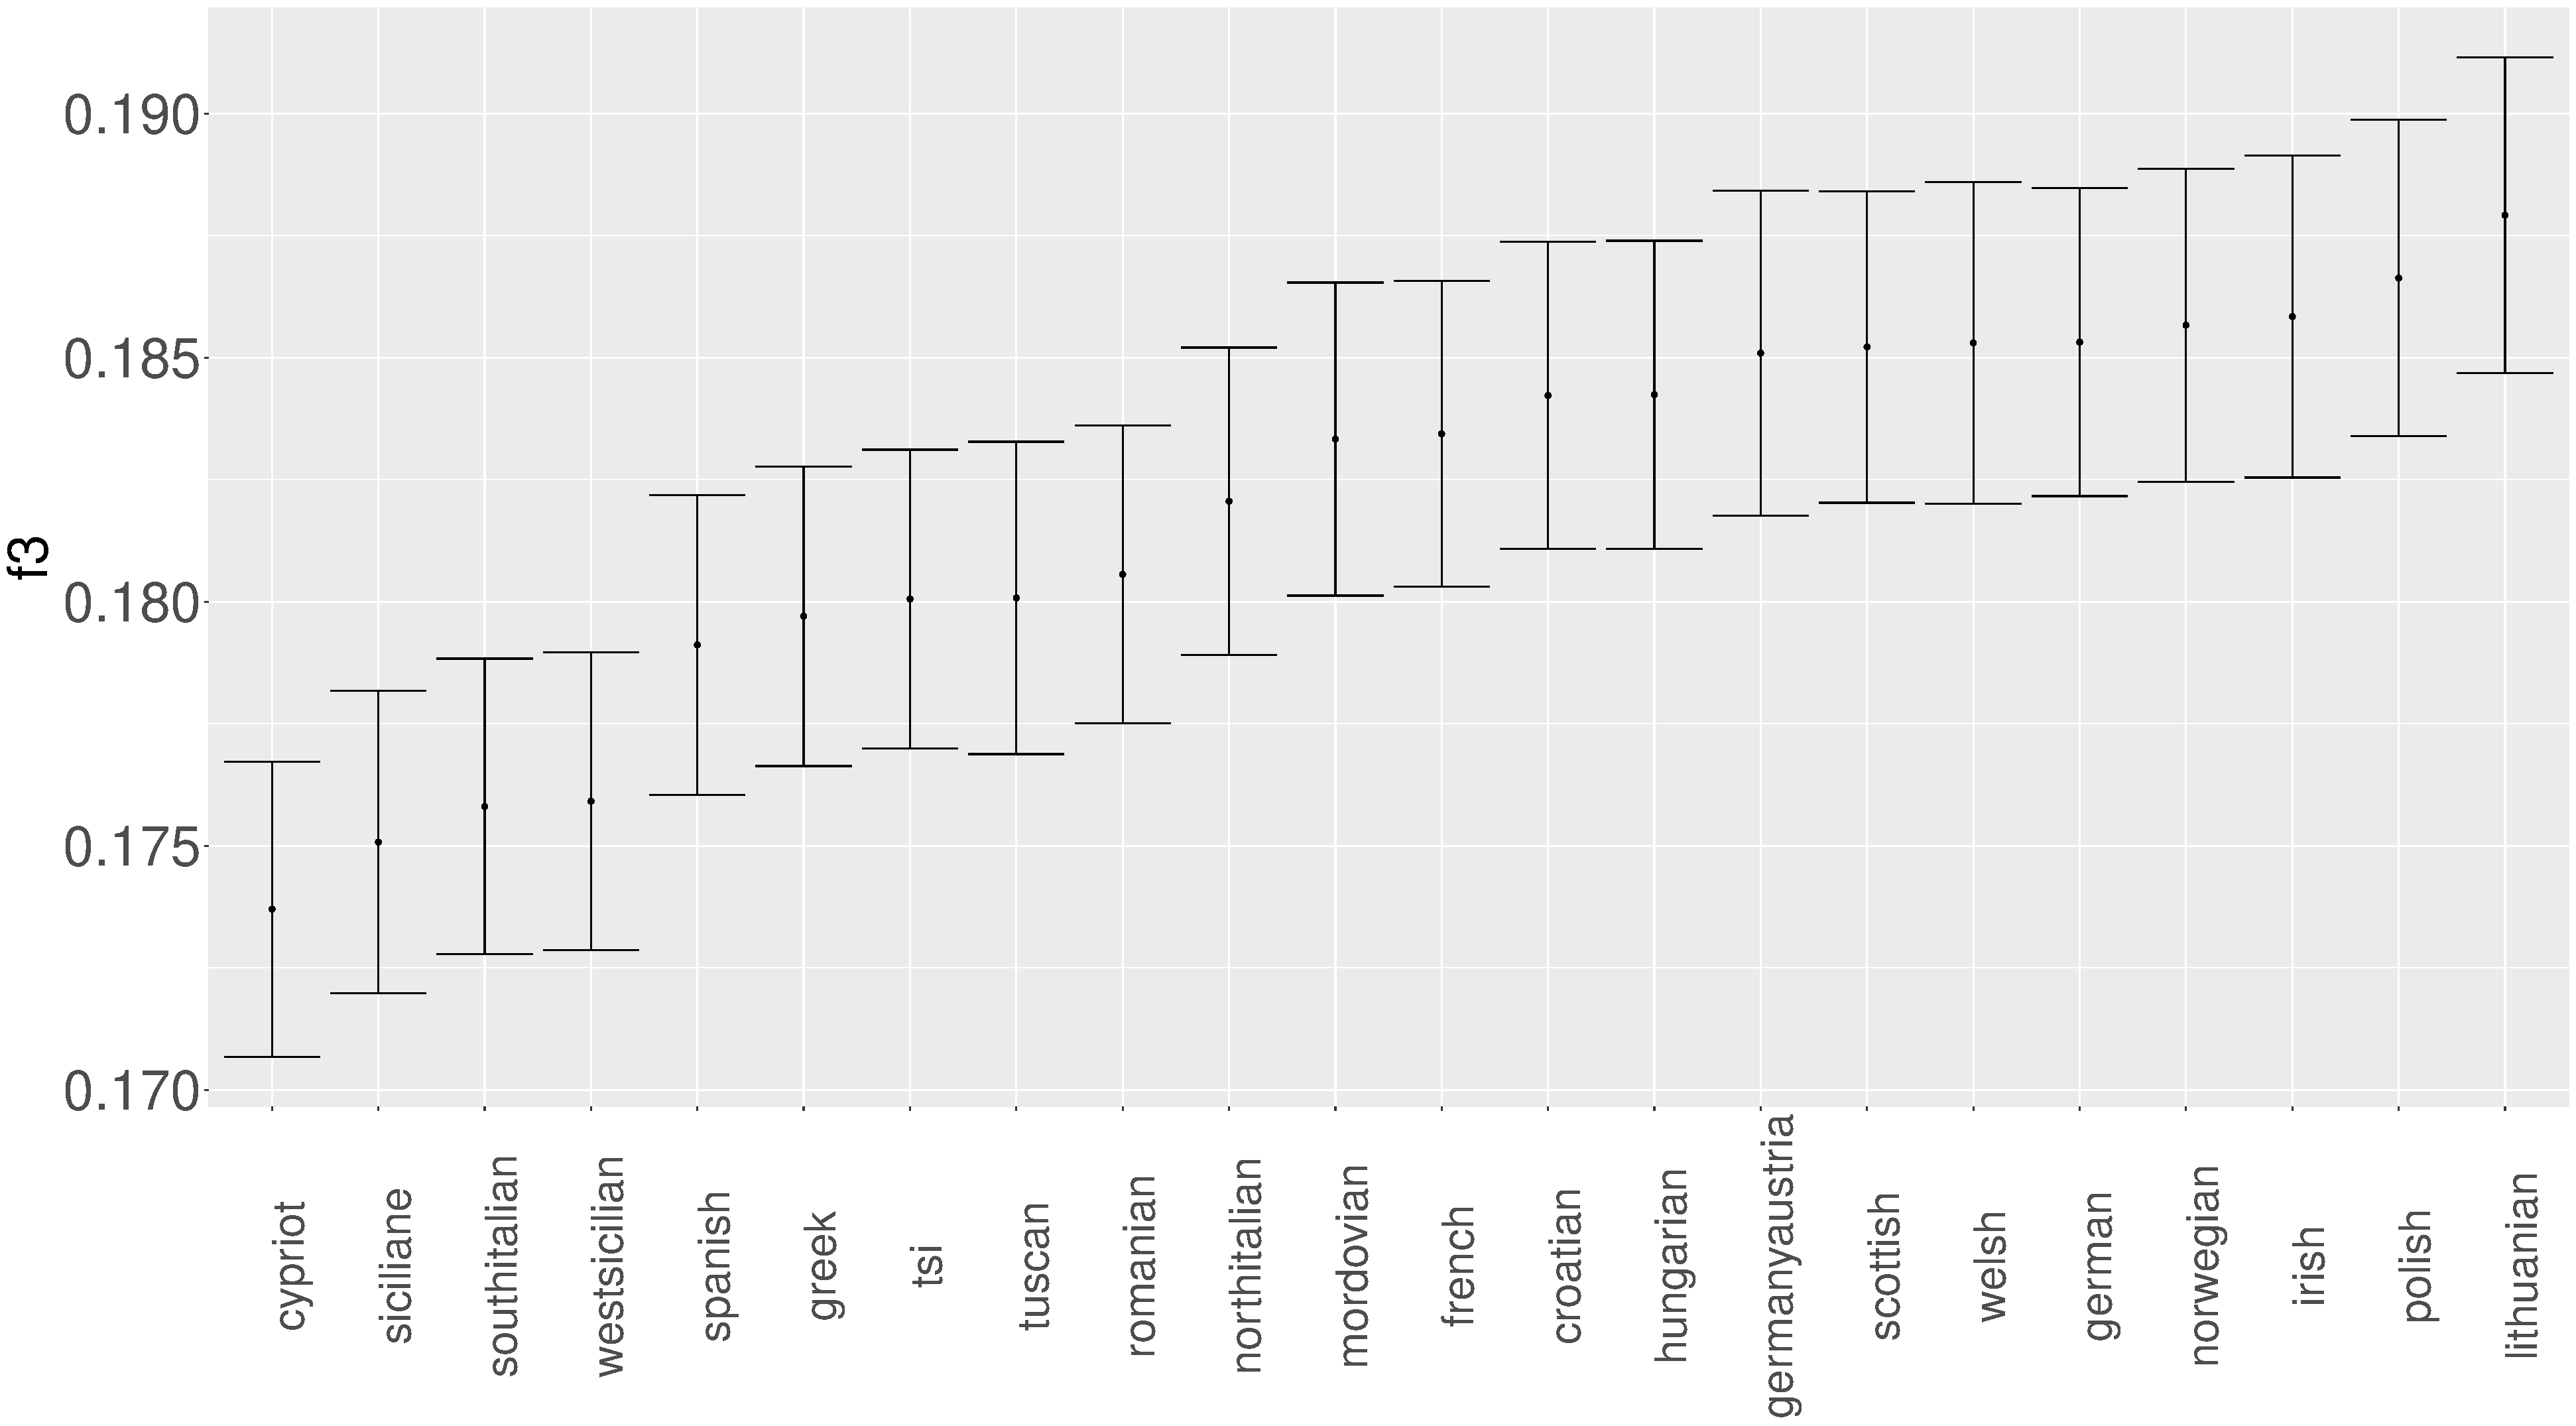
\includegraphics[width=1.0\textwidth]{../images/chapter5/f3_HB_ancient_slavs.pdf}
    \caption{$f_{3}$ statistics in the form of $f_{3}(EMA, present-day;mbuti pygmy$), where \textit{present-day} is different present-day European population. Error bars rerpesent $\pm*2$ stderr.}
    \label{fig:f3_HB_ancient_slavs}
\end{figure}

\subsection{Continuity with present-day day Slavs}

The previous section strongly suggests at least some degree of continuity between Early Middle Age samples and present day Slavic populations that is not shared with the samples from the Migration Period, as the Early Middle Age samples share many more haplotypes with present-day Slavs compared to Migration Period. 

To explicitly test the hypothesis that the Early Middle Age samples were continuous with the present-day day Slavic populations, I used \textit{qpWave}, which tests the number of streams of ancestry from a set of \textit{right} populations into a set of \textit{left} populations, $qpWave(left=croatian,lithuanian,polish,ukrainian, right=middleage,migration)$. The matrix with rank $r=0$ can be rejected ($p=0.112$). Note - not sure how to interpret this. 

\begin{figure}[htp]
    \centering
    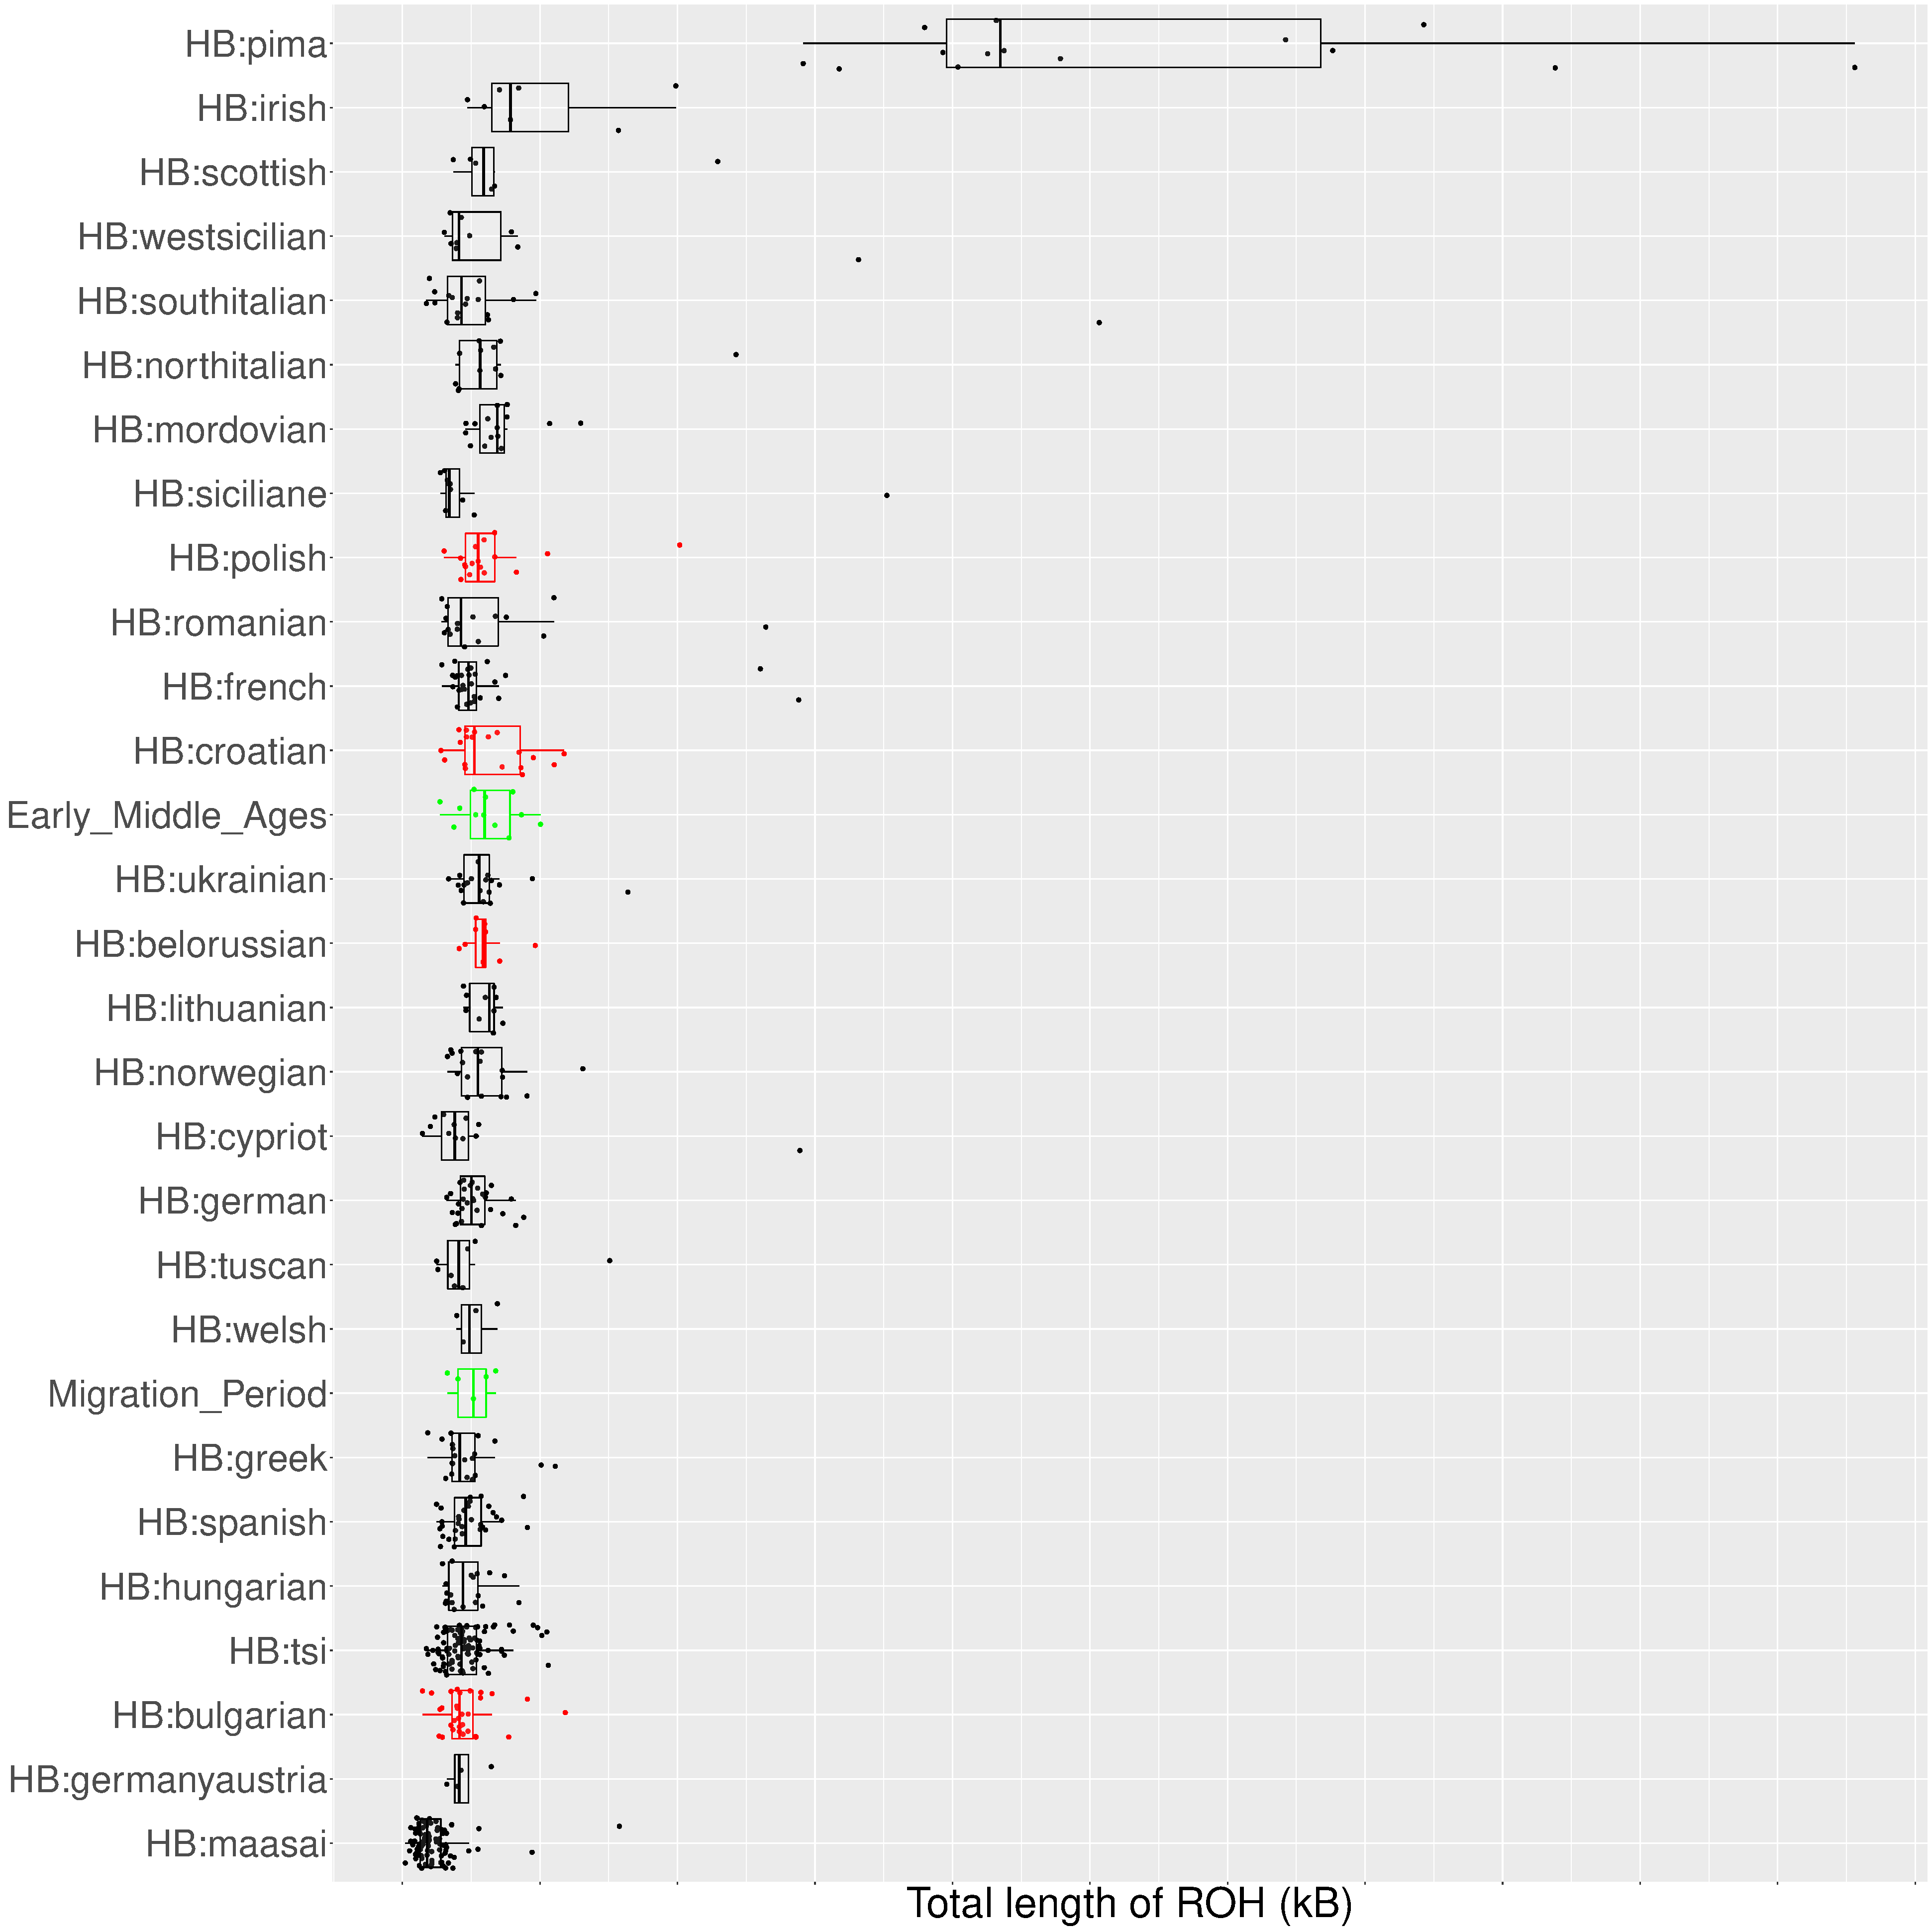
\includegraphics[width=1.0\textwidth]{../images/chapter5/ROH_plot.pdf}
    \caption{Total length of runs-of-homozygosity (ROH) in different present-day and ancient populations. Each point is the total length of ROH (kB) within an individual in that population. Points given jitter to aid visualisation. HB:pima and HB:masasai included to display extremes of ROH in different present-day human populations.}
    \label{fig:ROH}
\end{figure} 

\subsection{Genetic structure and admixture events of present-day Slavic people}

As described in the introduction, several studies have looked at the structure of present-day Slavic populations, but none have integrated autosomal DNA from present-day and ancient samples and analysed them jointly with haplotype-based methods. I performed an all-v-all painting of a selection of present-day European populations and all newly sequenced ancient Slavic samples and applied the fineSTRUCTURE algorithm to the resulting chunkcounts matrix, inferring 32 clusters.

As a whole, present-day Slavs do not form a monophyletic group within the fineSTRUCTURE dendrogram to the exclusion of non-Slavic populations (Fig. \ref{fig:tree_with_ancients}), as several non-Slavic speaking populations such as German, Irish and Scottish cluster in the main clade containing Slavic speakers. However, some structure is apparent; speakers of `Southern' Slavic languages from Croatia and Bulgaria form a group to the exclusion of 'Eastern' Slavic speaking populations from Belarus, Russia and Ukraine. Individuals from Poland cluster with `Eastern' Slavic speakers, suggesting the principle axis of variation splits populations into `North-West' and `South-East' groups. 

\begin{figure}[htp]
    \centering
    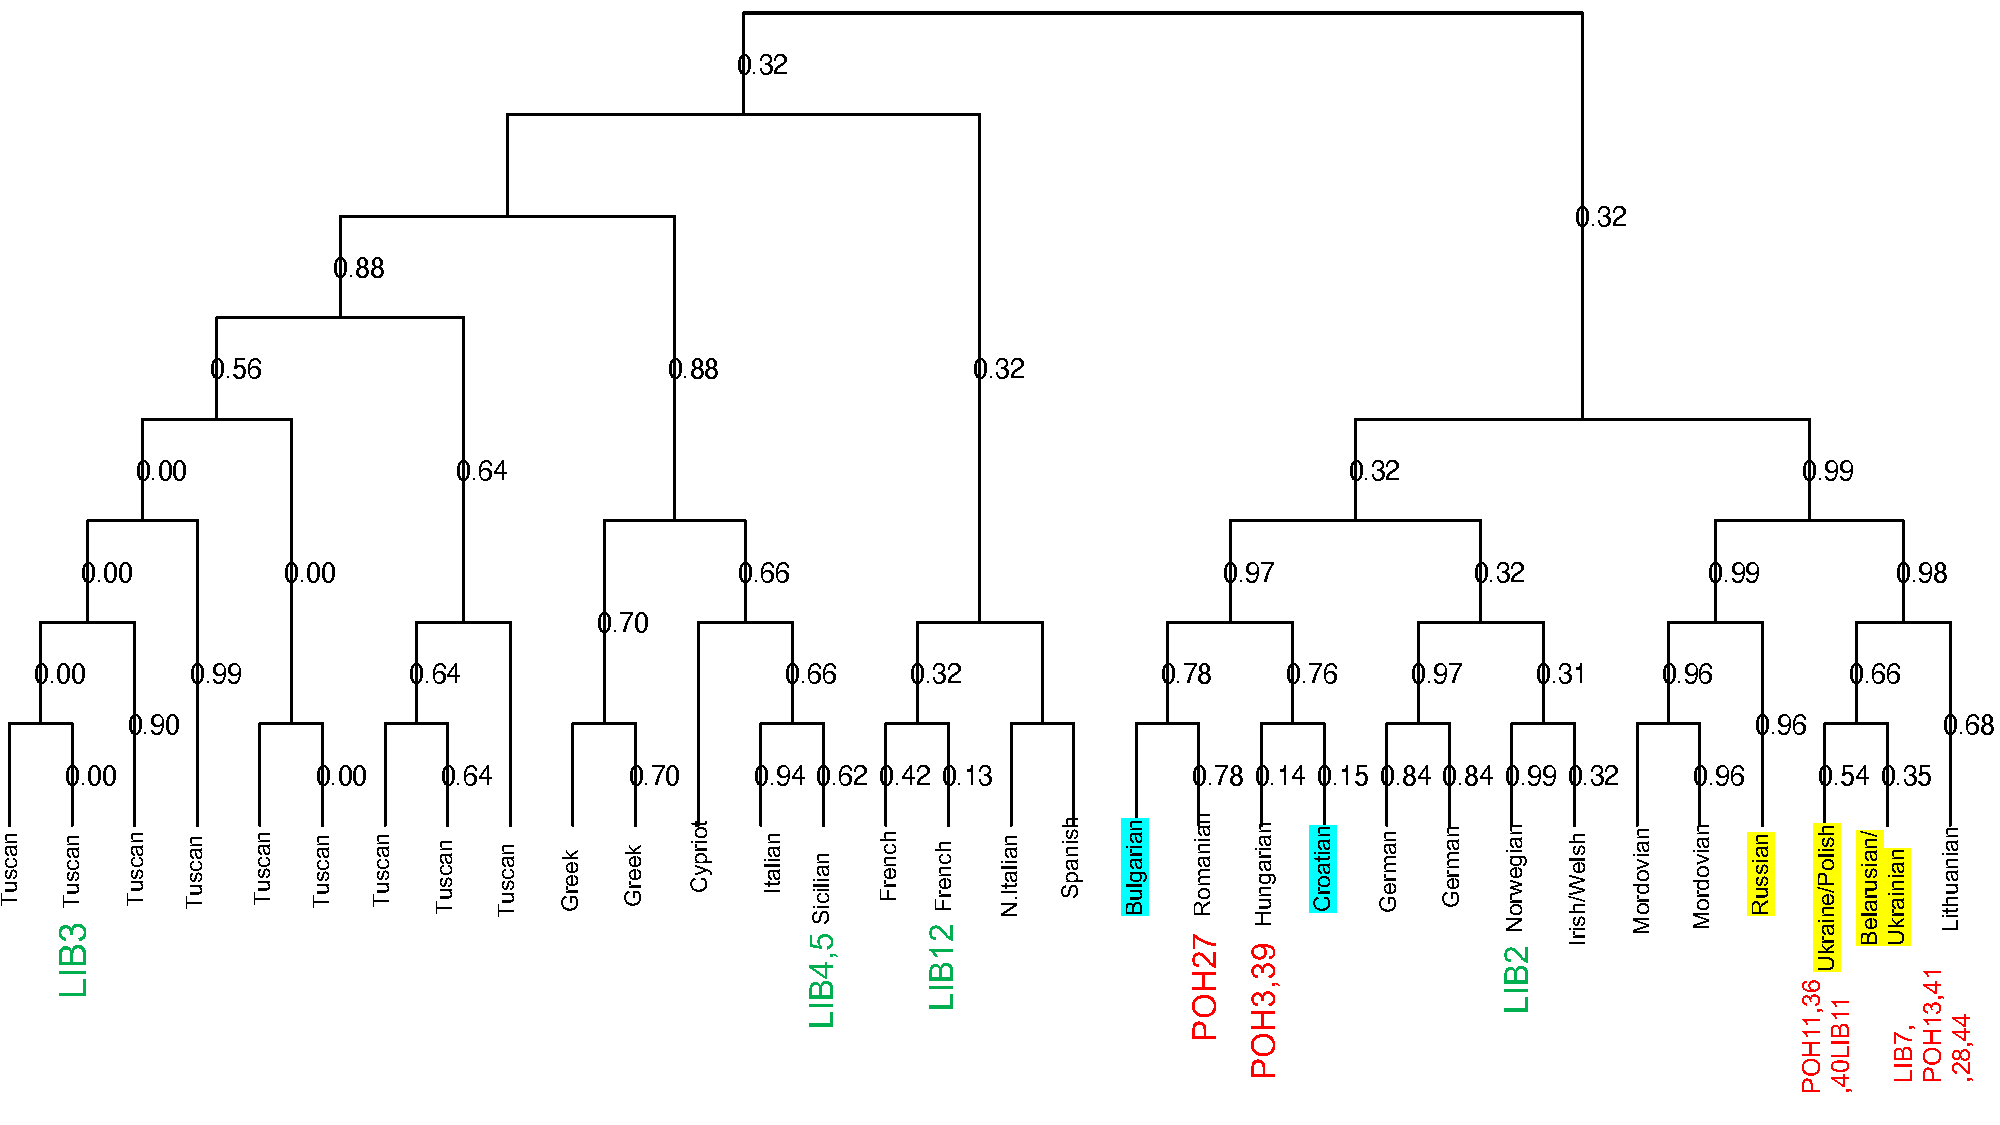
\includegraphics[width=1.0\textwidth]{../images/chapter5/tree_with_ancients.pdf}
    \caption{Population dendrogram generated by the fineSTRUCTURE tree building algorithm. Labeled tips refer to the primary population(s) represented in that clade. present-day non-Slavic populations shown in black. `South-East' Slavs highlighted in cyan and `North-West' Slavs highlighted in yellow. Migration period individuals superimposed in green and Early Middle Age samples superimposed in red. Read fineSTRUCTURE paper for description of edge values. Note: some tips contained more than one population but were not included as labels to save space.}
    \label{fig:tree_with_ancients}
\end{figure} 

Of the Early Middle Age samples, 3 samples (POH3, POH39, POH27) were present in the `South-East' Slavic cluster, falling into a group composed of Bulgarian and Romanian samples. The remaining 7 samples are found in the `North-West' cluster containing samples from Lithuania, Poland, Ukraine and Belarus. Painting the samples using present-day individuals has thus uncovered structure that was not able to be detected by looking only at ancient samples. It also suggests the structure of Slavic populations into was present at least as early as the date of these samples. 

Previous studies have identified admixture events in present-day Slavic populations involving an East Asian source approximately xx years ago \cite{Hellenthal2016, MOSAIC_2019}. In previous sections, I showed that this signal exists in the Early Middle Age ancient samples, best characterised by populations from present-day Mongolia (Fig. \ref{fig:EarlyMiddleAges_MOSAIC_3way_moderns_Mu}). 

I employed MOSAIC to replicate these results and determine whether a similar admixing source is present in the ancient populations. 

When considering 2-way admixture event, all of the tested populations, bar the Migration Period Slavs, showed evidence of an admixture event involving a minor source which has the lowest Fst with present-day  Uygurs. The dates and bootstrapped confidence intervals are given in Fig.  \ref{fig:MOSAIC_admixture_dates_plot}. 

\begin{figure}[htp]
    \centering
    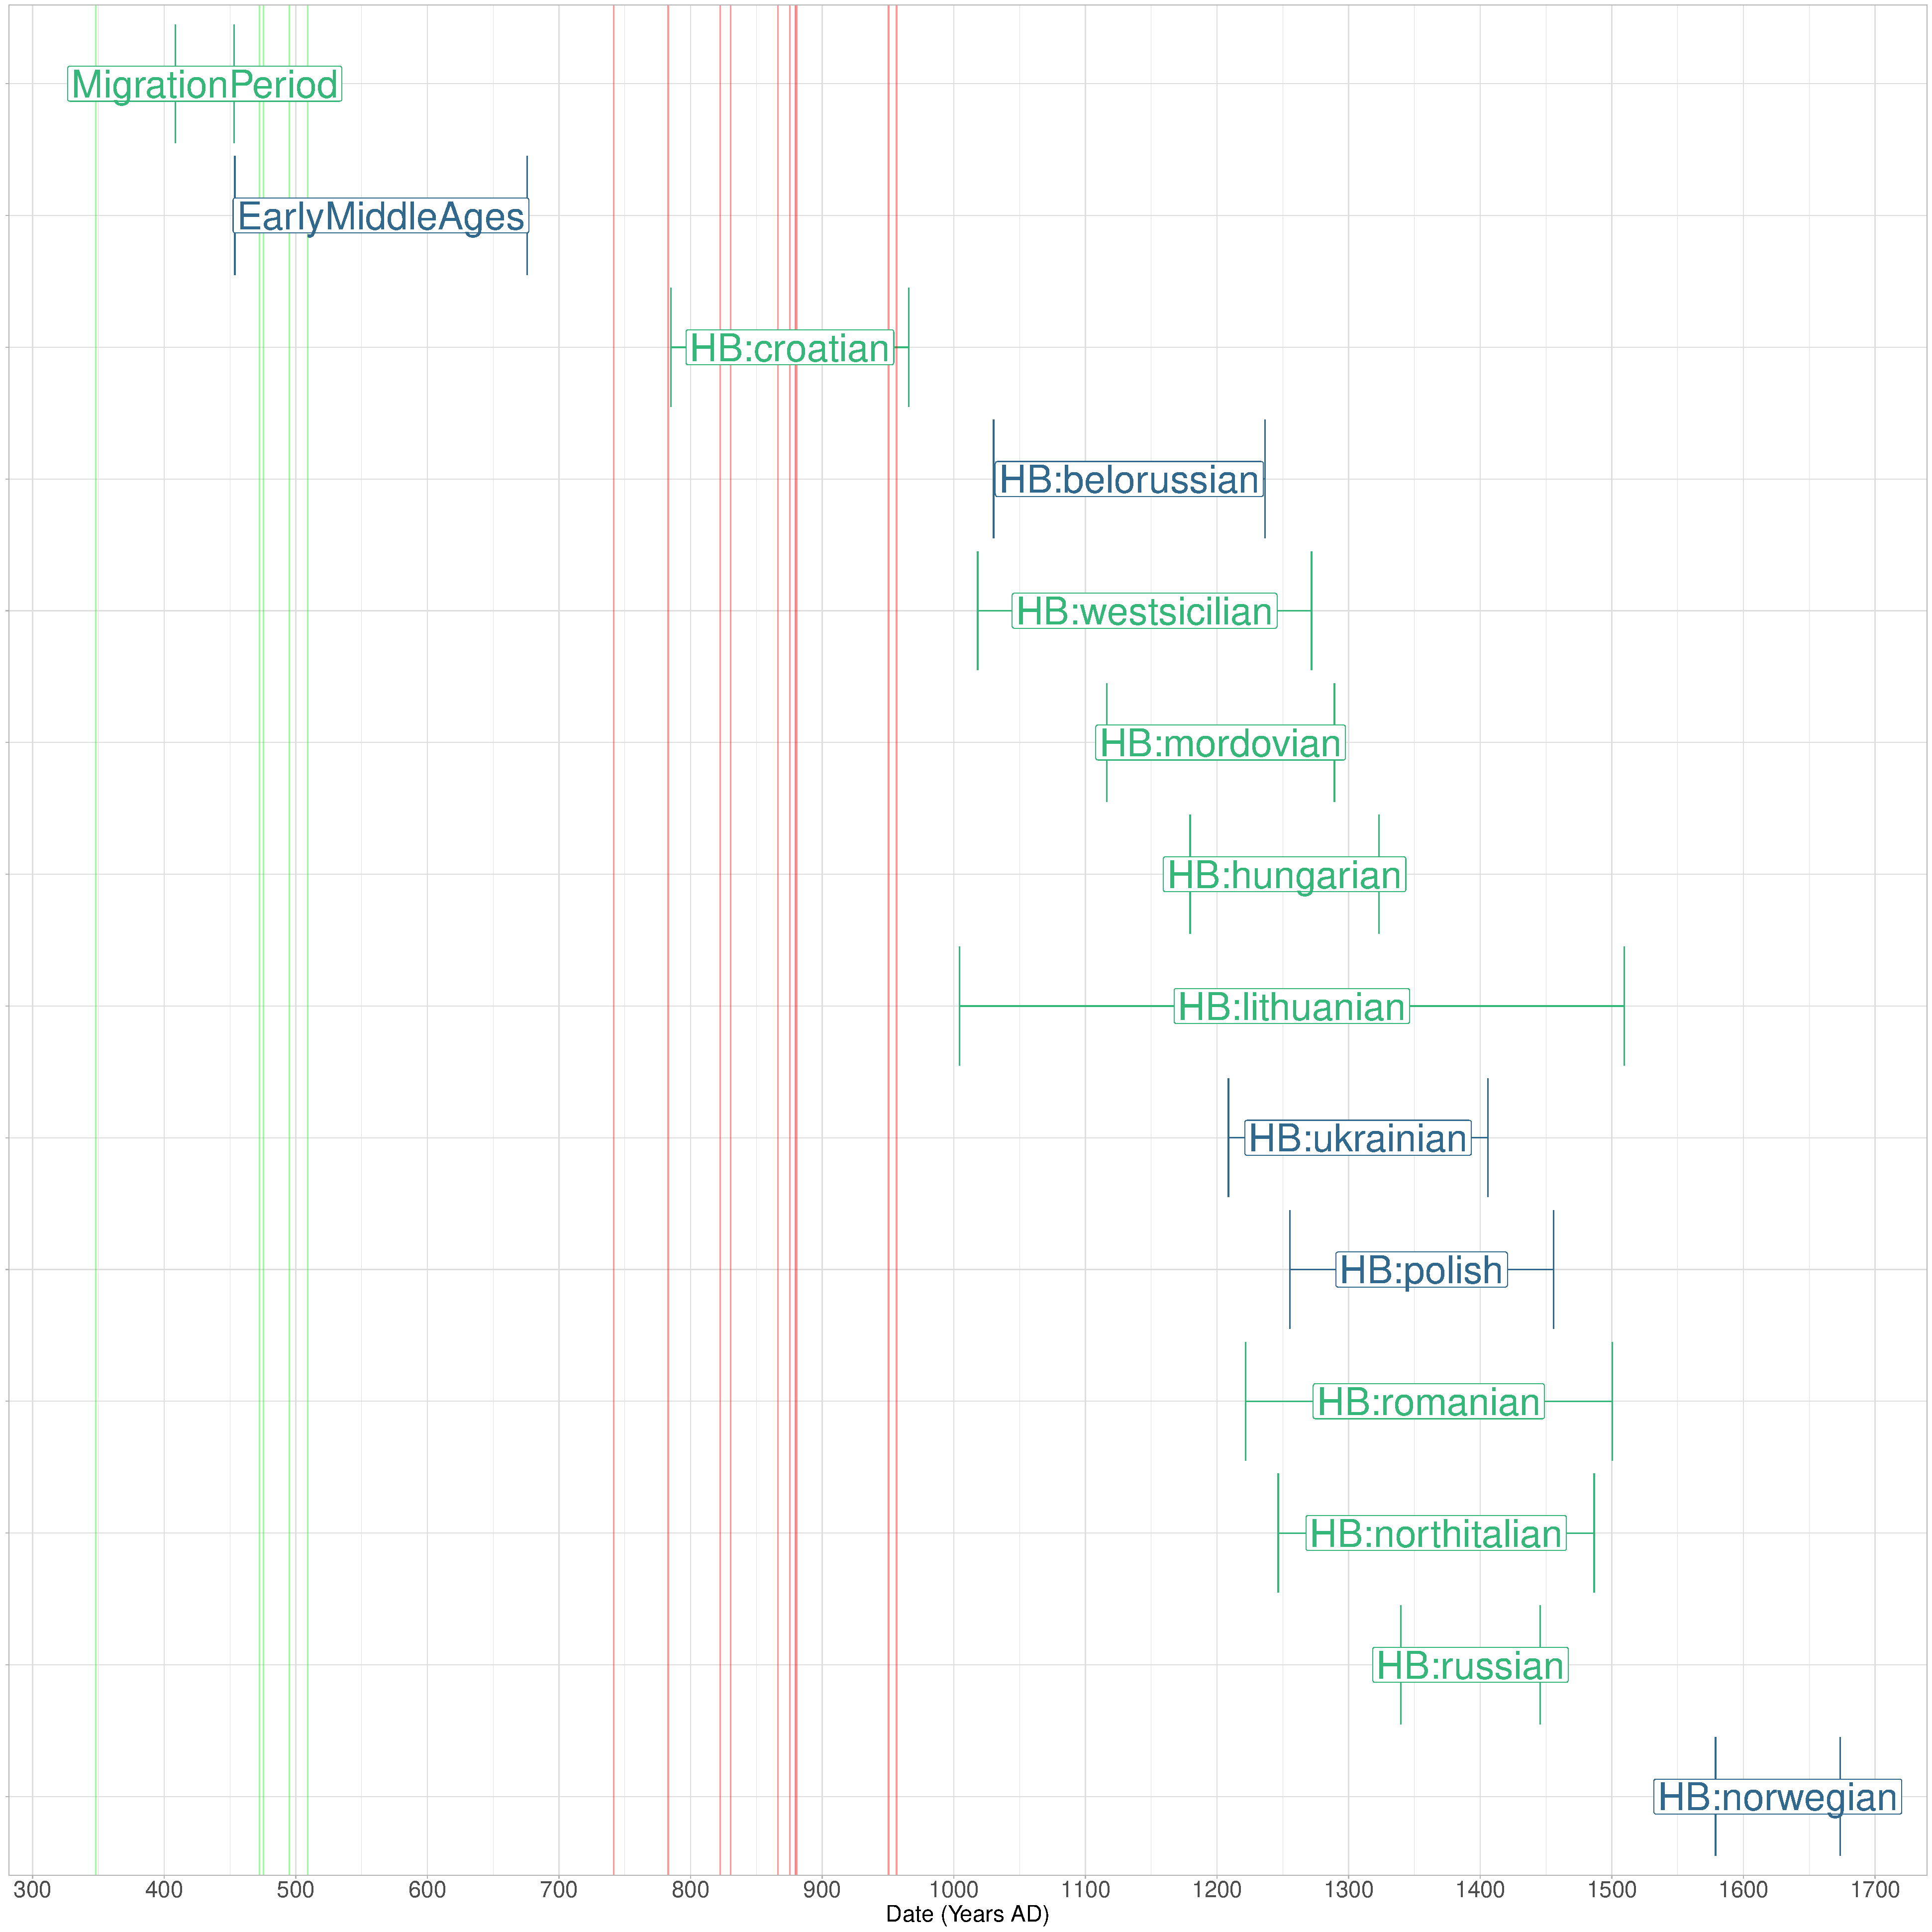
\includegraphics[width=1.0\textwidth]{../images/chapter5/MOSAIC_admixture_dates_plot.pdf}
    \caption{MOSAIC inferred 2-way admixture dates with bootstrapped 97.5\% and 2.5\% CI. Vertical green lines correspond to radiocarbon estimated dates of Migration Period samples and red lines equivalent for Early Middle Age samples.}
    \label{fig:MOSAIC_admixture_dates_plot}
\end{figure} 

Interestingly, most present-day Slavic speaking populations, such as present-day Polish, show evidence of a 3-way admixture event, where the middle component has the lowest $F_{st}$ with Migration Era ancient samples (Fig. \ref{fig:Fst_plot_HB:lithuanian}). The major component has a low $F_{st}$ with Early Middle Age Slavs. This suggests that the formation of present-day Slavic populations could have occured via an admixture event(s) involving Migration Era individuals with high levels of Southern European ancestry, Middle Age Era samples which show a strong affinity to present day Eastern Europeans, and a small but significant East Asian source best represented by present-day Uygurs. 


\begin{figure}[htp]
    \centering
    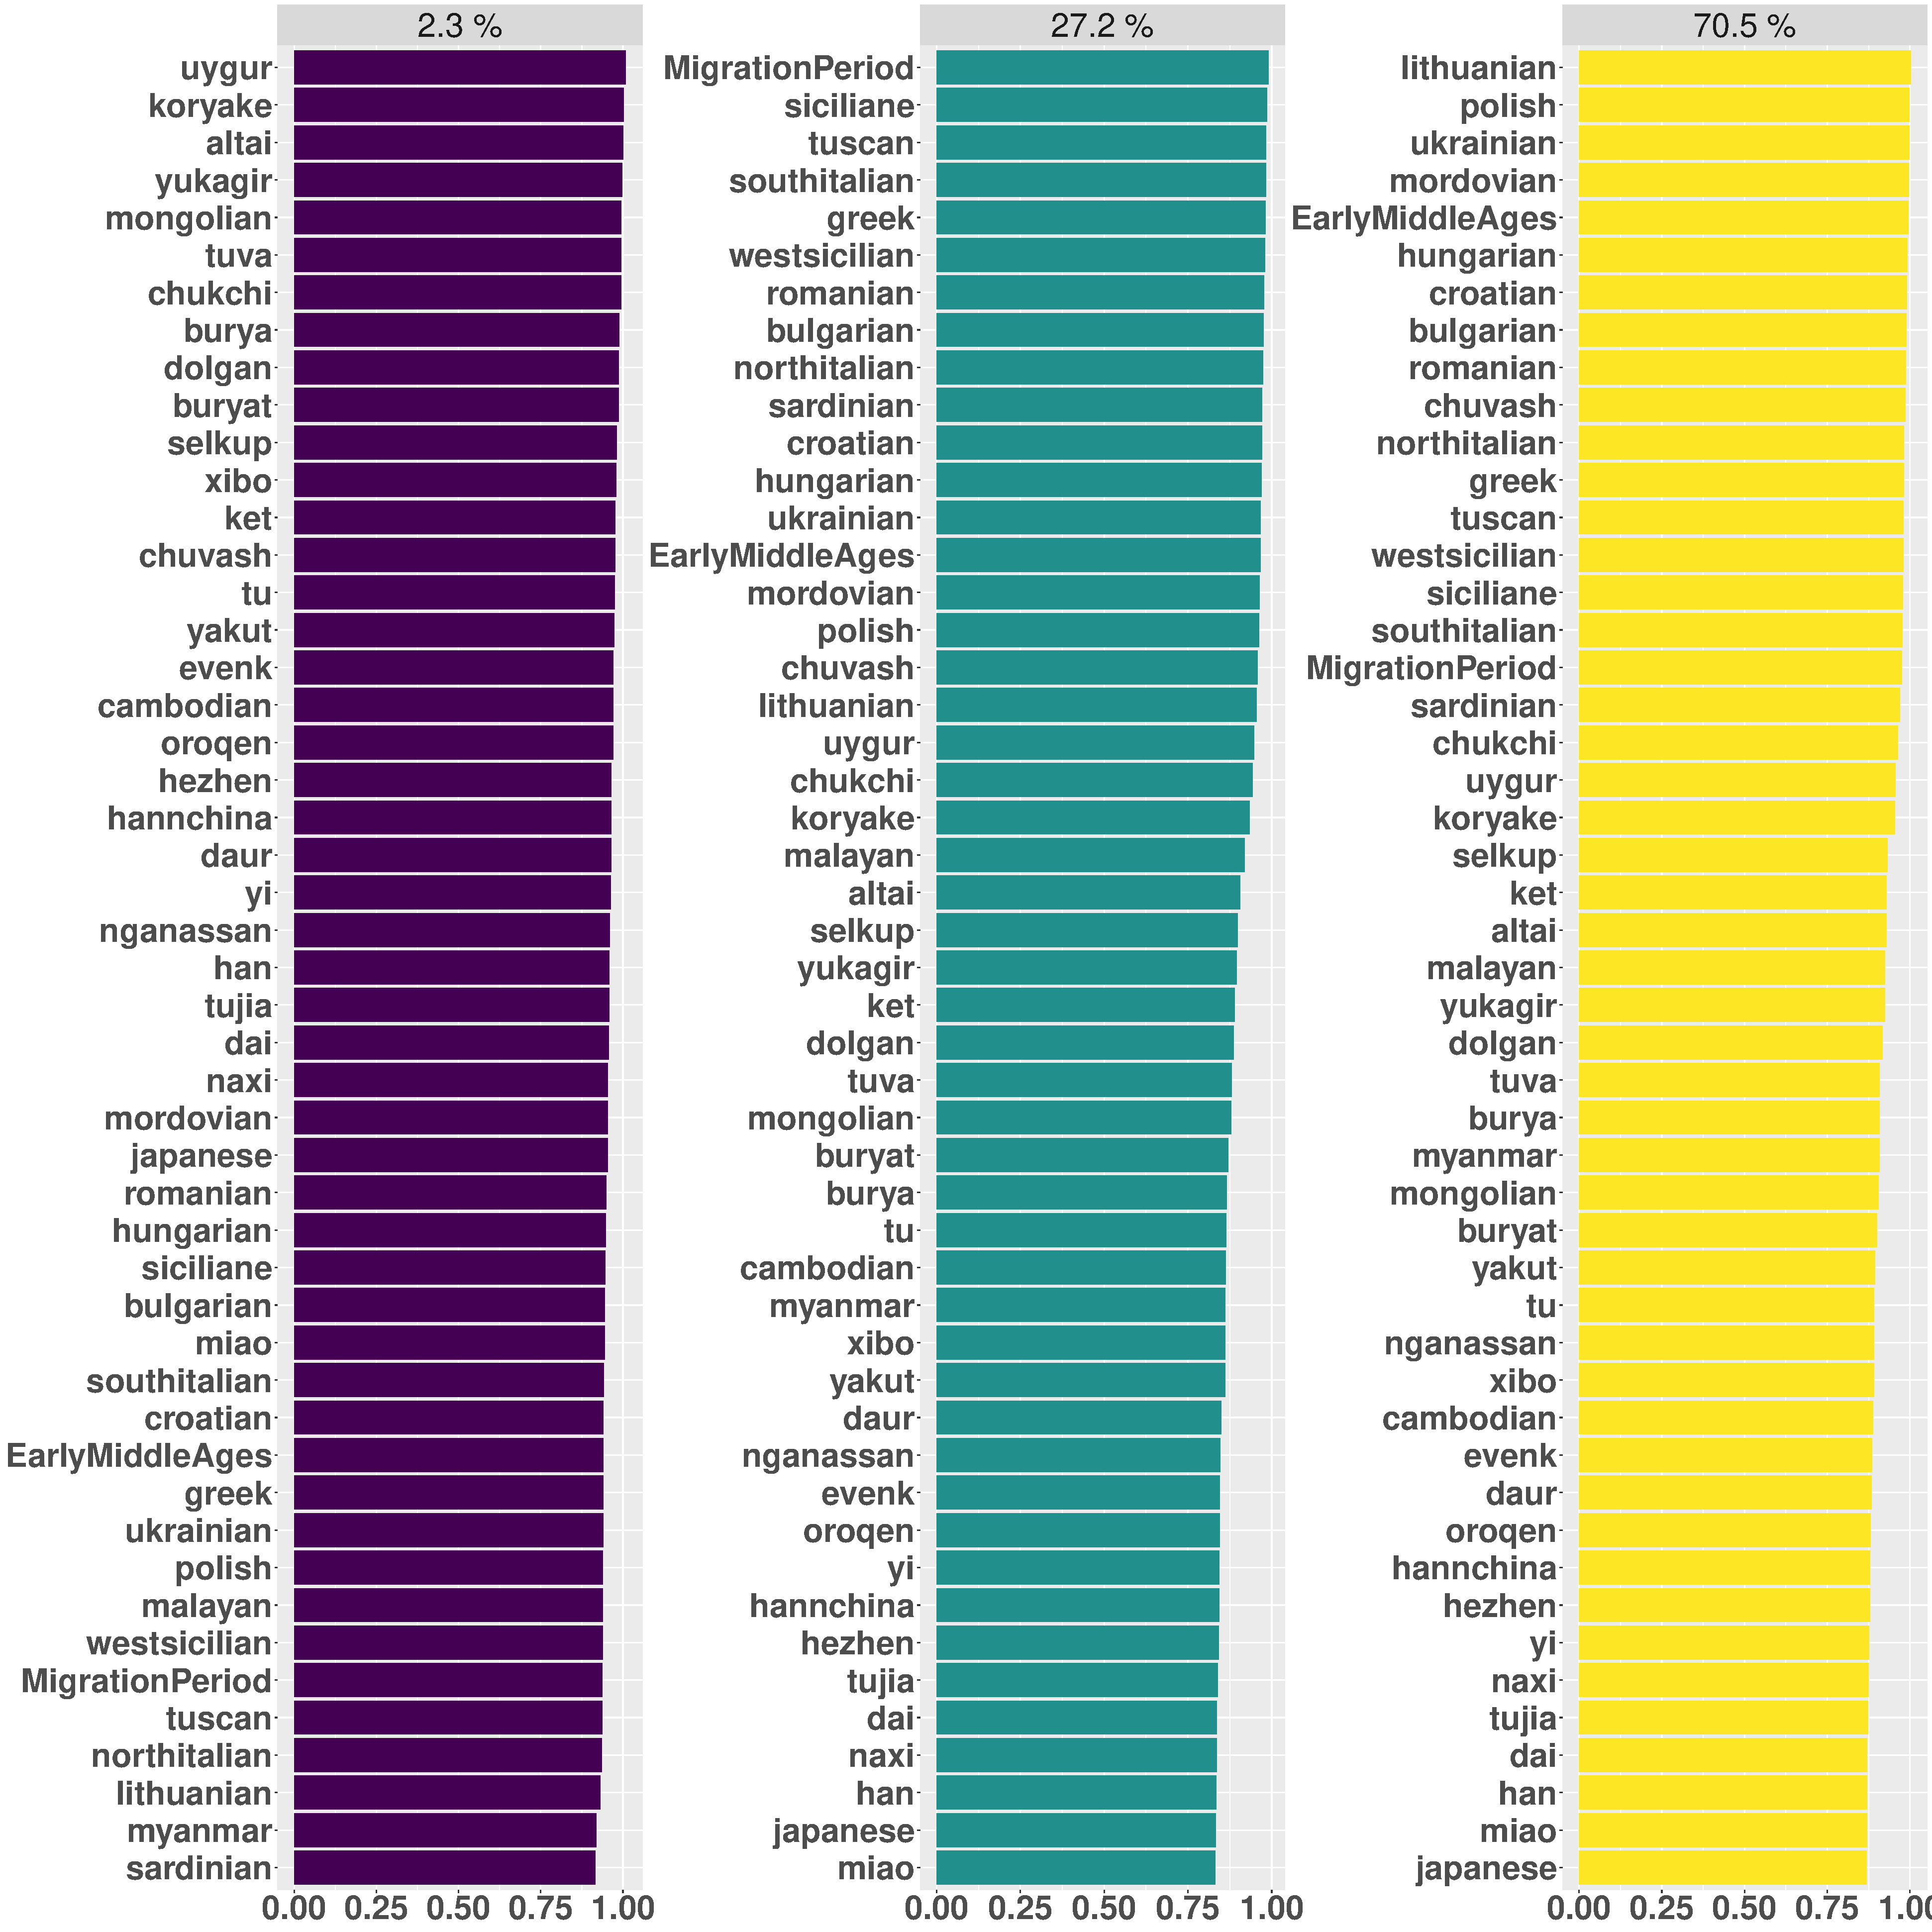
\includegraphics[width=1.0\textwidth]{../images/chapter5/Fst_plot_HB:belorussian.pdf}
    \caption{$1 - F_{st}$ between 3 inferred mixing sources for present-day Belorussians. Each panel represent a different mixing source. Each bar gives the value $1-F_{st}$ between that samples population and the mixing source. Higher values of $1-F_{st}$ suggest that source is well represented by a particular population. }
    \label{fig:Fst_plot_HB:lithuanian}
\end{figure} 

\section{Discussion}

The combined results from the Migration Period suggest the individuals living in Czechia during this time period were of mixed ancestry and did not originate from the same source population. The diverse set of ancestries, spanning from Scandinavia to Southern Europe imply that the Migration Period was truly a period of Migration where individuals from distal ends of Europe lived among one another. I identified ancestry sources from Southern Europe and Scandinavia. 

The results from the analysis of combined ancient and present-day genomes are consistent with those from Kushniarevich et al (2015) \cite{Kushniarevich23015} who determined that Eastern (Russia, Belarus, Ukraine) and Western (Polish) central European Slavs form a cluster to the exclusion of Southern Slavs (Croatia, Bulgaria), whilst also remaining distinct from geographically proximate Germanic (German/Austrian) and Baltic (Lithuanian) populations. This is also consistent with results from Veeramah et al 2011, who showed that Sorbs, a west-Slavic population found between Poland and Germany, have a much stronger affinity to more distant Slavic populations from Czechia than to more proximate Germans \cite{veeramah2011genetic}. Similarly, I found that the Slavisiation of the Balkan peninsula doesn't extend beyond Croatia; the cluster of Croatian individuals only derives 1.2\% of their ancestry from nearby Greek sources. However, admixture modeling suggested that Southern Slavs show signals of a historic admixture event where the minor source is related to present-day Mediterranean populations. An admixture event with a similar minor source is found in Migration period samples, albeit dated further in the past. 

I recapitulated a previously described admixture event into not only present day Slavic speaking populations, but also Southern Europeans (e.g. North Italians). The source of this East-Asian admixture is most clost to present-day Uygurs. However, the true ancient population that was repsonsible to transmitting East-Asian ancestry into Europe is yet to be determined. It seems likely that the ancestry was brought to Europe via an intermediate population containing East Asian ancestry, such as the Huns or Turkic peoples. 

